\chapter{Stimuli for perception experiments}\label{appen:stimuli}

\noindent This appendix provides additional information on the perception experiments described in Chapter \ref{ch:perc}.  First, example answersheets for each experiment and the production task are provided.  For the production task, participants read the sentences only once through.  There were no instructions provided.  

Next, the auditory tokens for each question are listed for each experiment, and they are labelled by type.  Due to the difficulty of finding stimuli for Experiment 1 that were matched at the lexical level, some tokens were used for more than one question.  It is possible that participants' exposure to the token the first time influenced their response to that token the second time.  However, the results do not seem to be dependent on such an effect as they were replicated in Experiment 2 where there were no re-plays of tokens across different questions that compared the same functions.

%don't think this is a problem b/c no effect from first to second half (this argument is shite)



\begin{figure}[htbp]
	\centering
		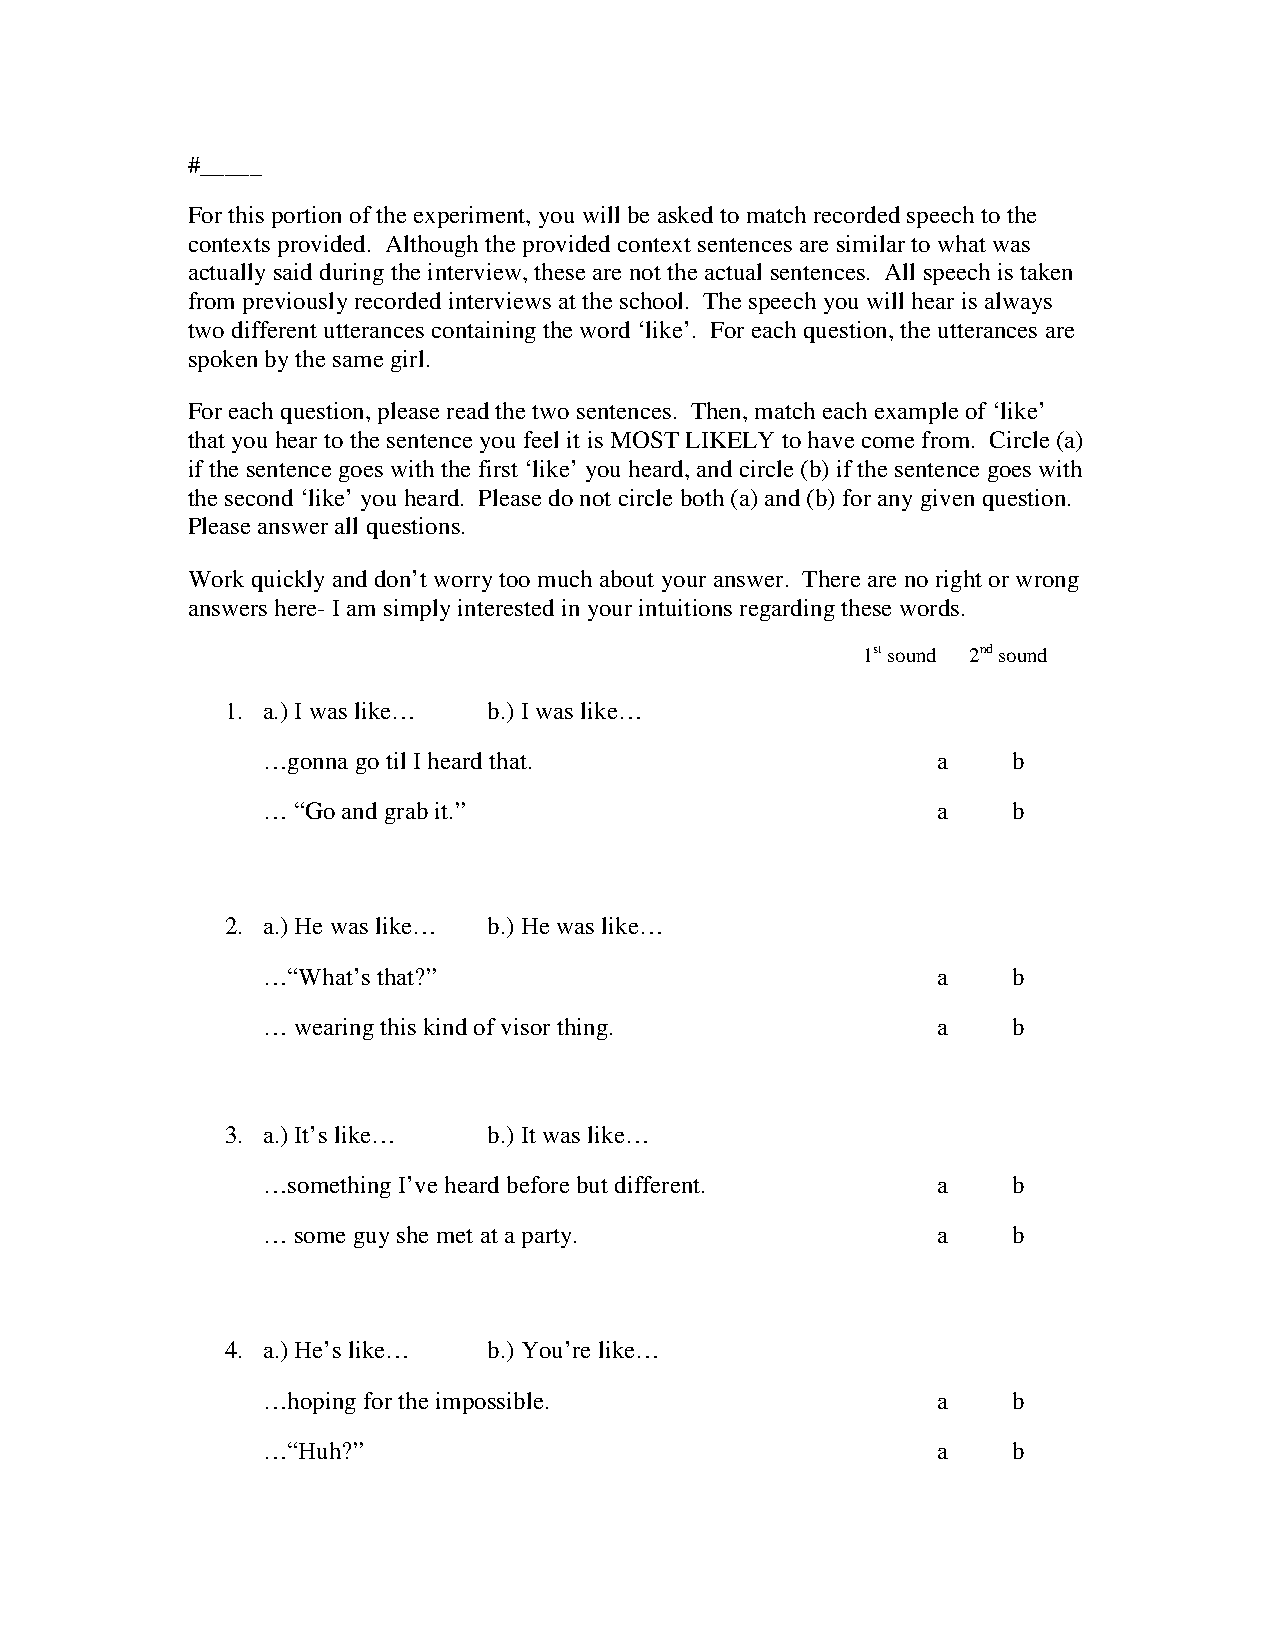
\includegraphics[width=5in]{images/Exp1page1.pdf}
		\caption{Answersheet for Experiment 1}
		\label{x1p1}
\end{figure}

\begin{figure}[htbp]
	\centering
		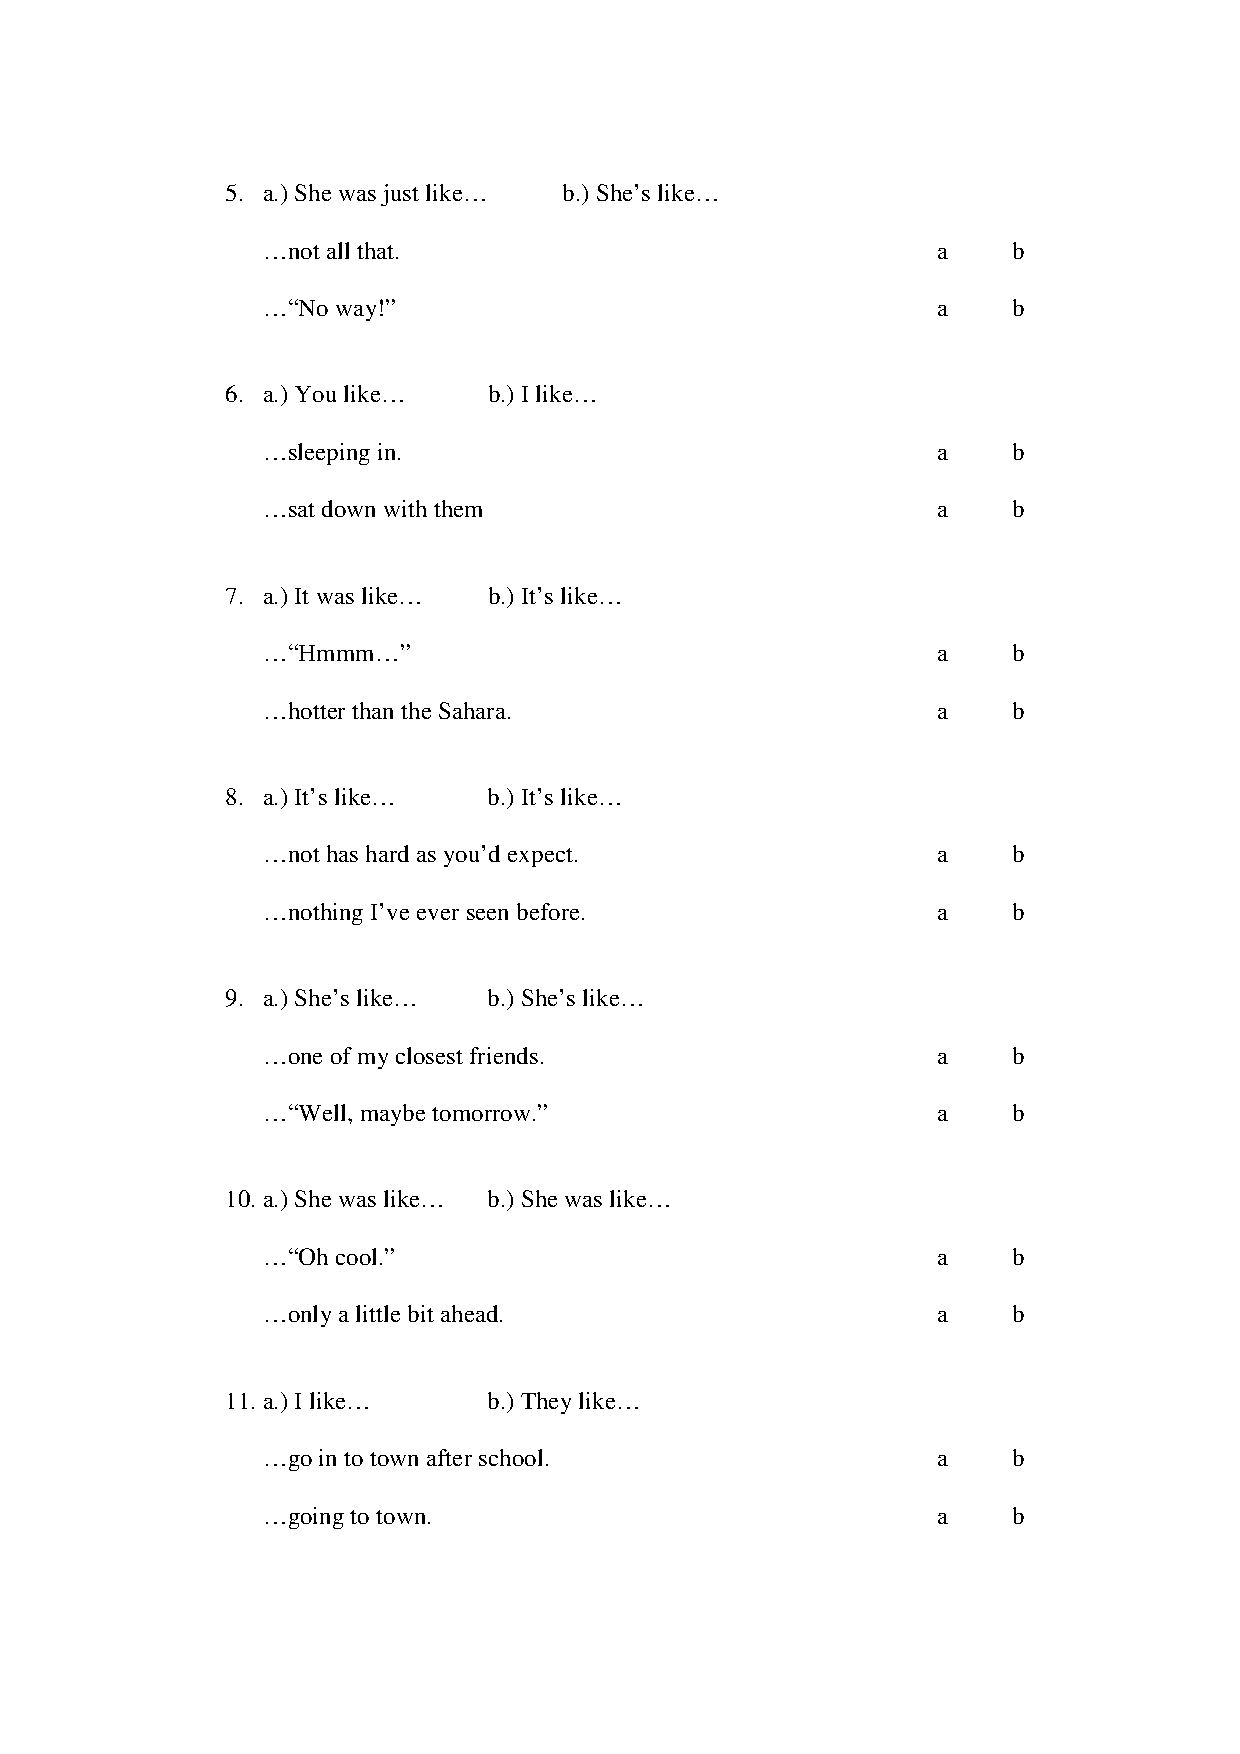
\includegraphics[width=5in]{images/Exp1page2.pdf}
		\label{x1p2}
\end{figure}

\begin{figure}[htbp]
	\centering
		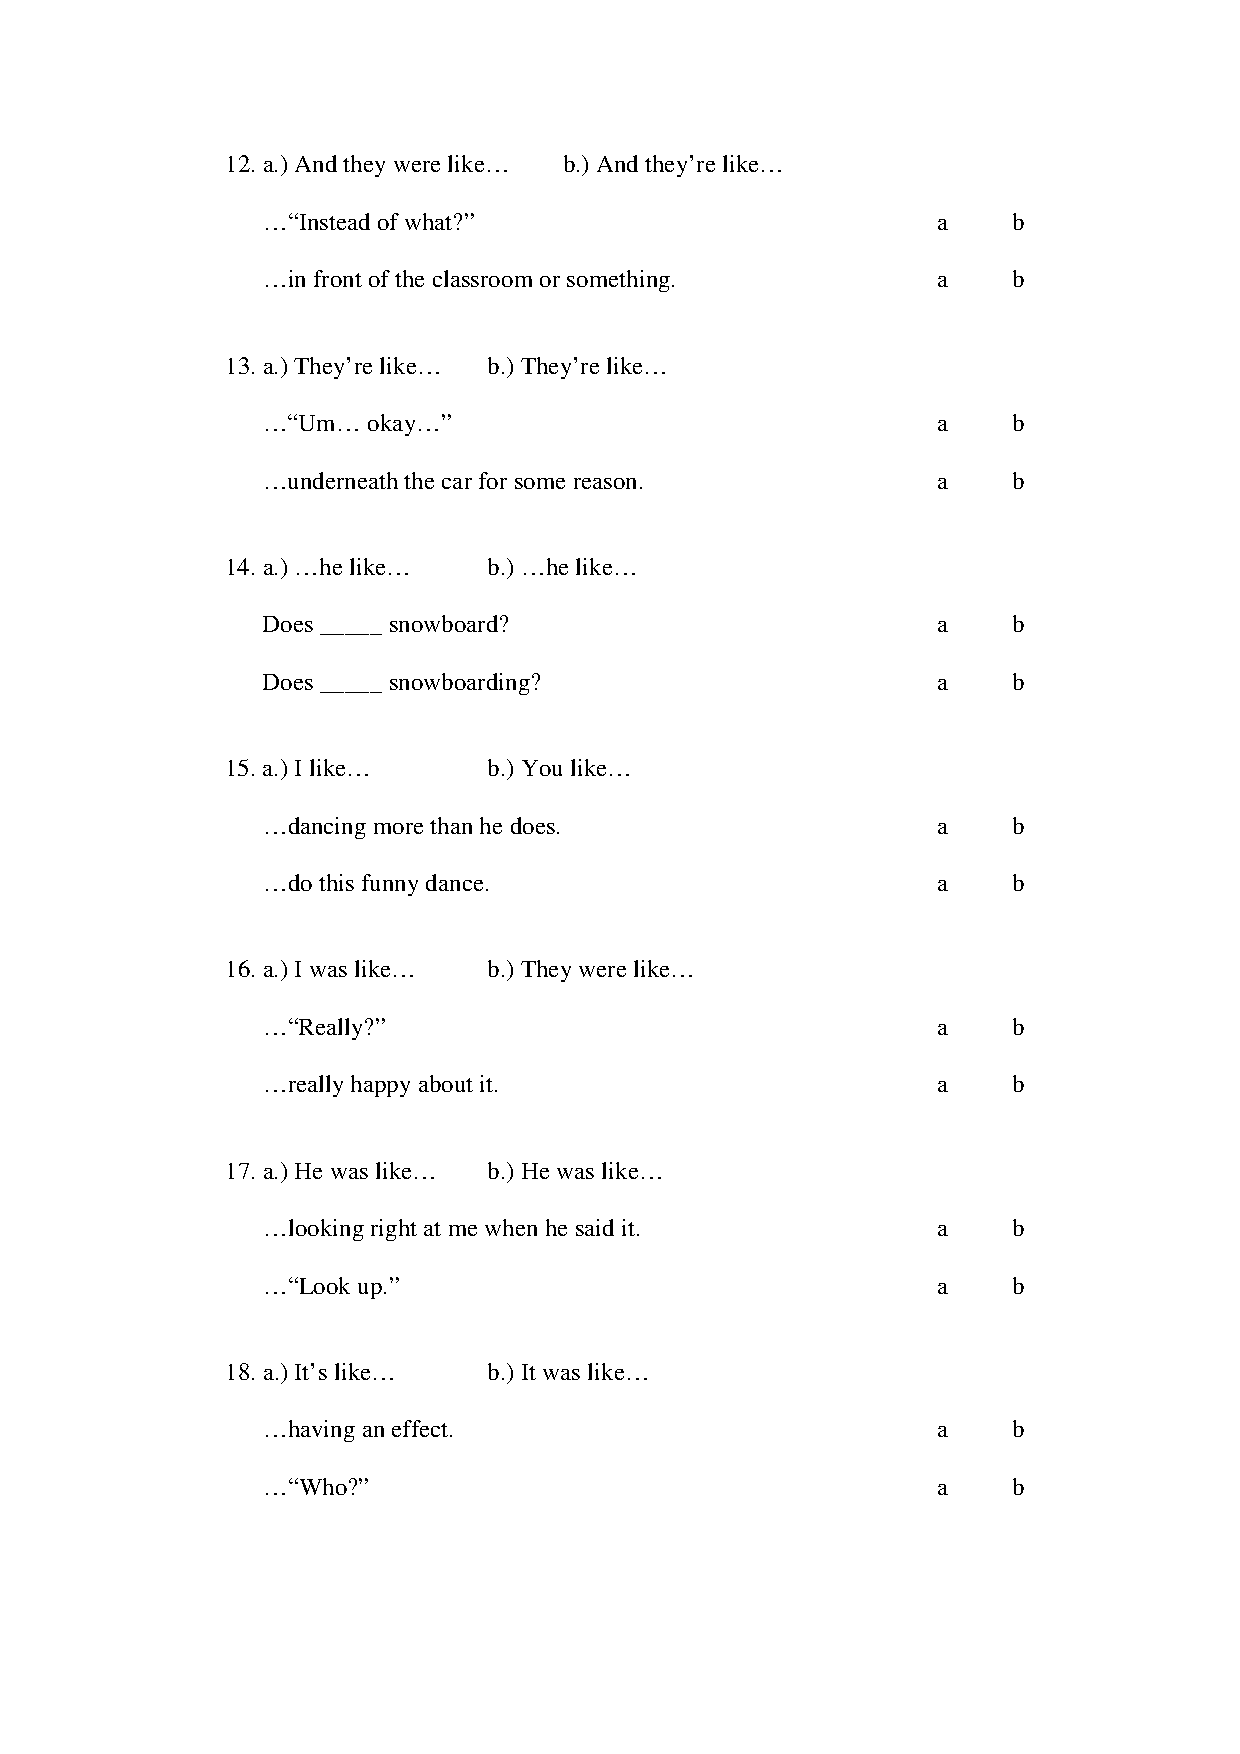
\includegraphics[width=5in]{images/Exp1page3.pdf}
		\label{x1p3}
\end{figure}

\begin{figure}[htbp]
	\centering
		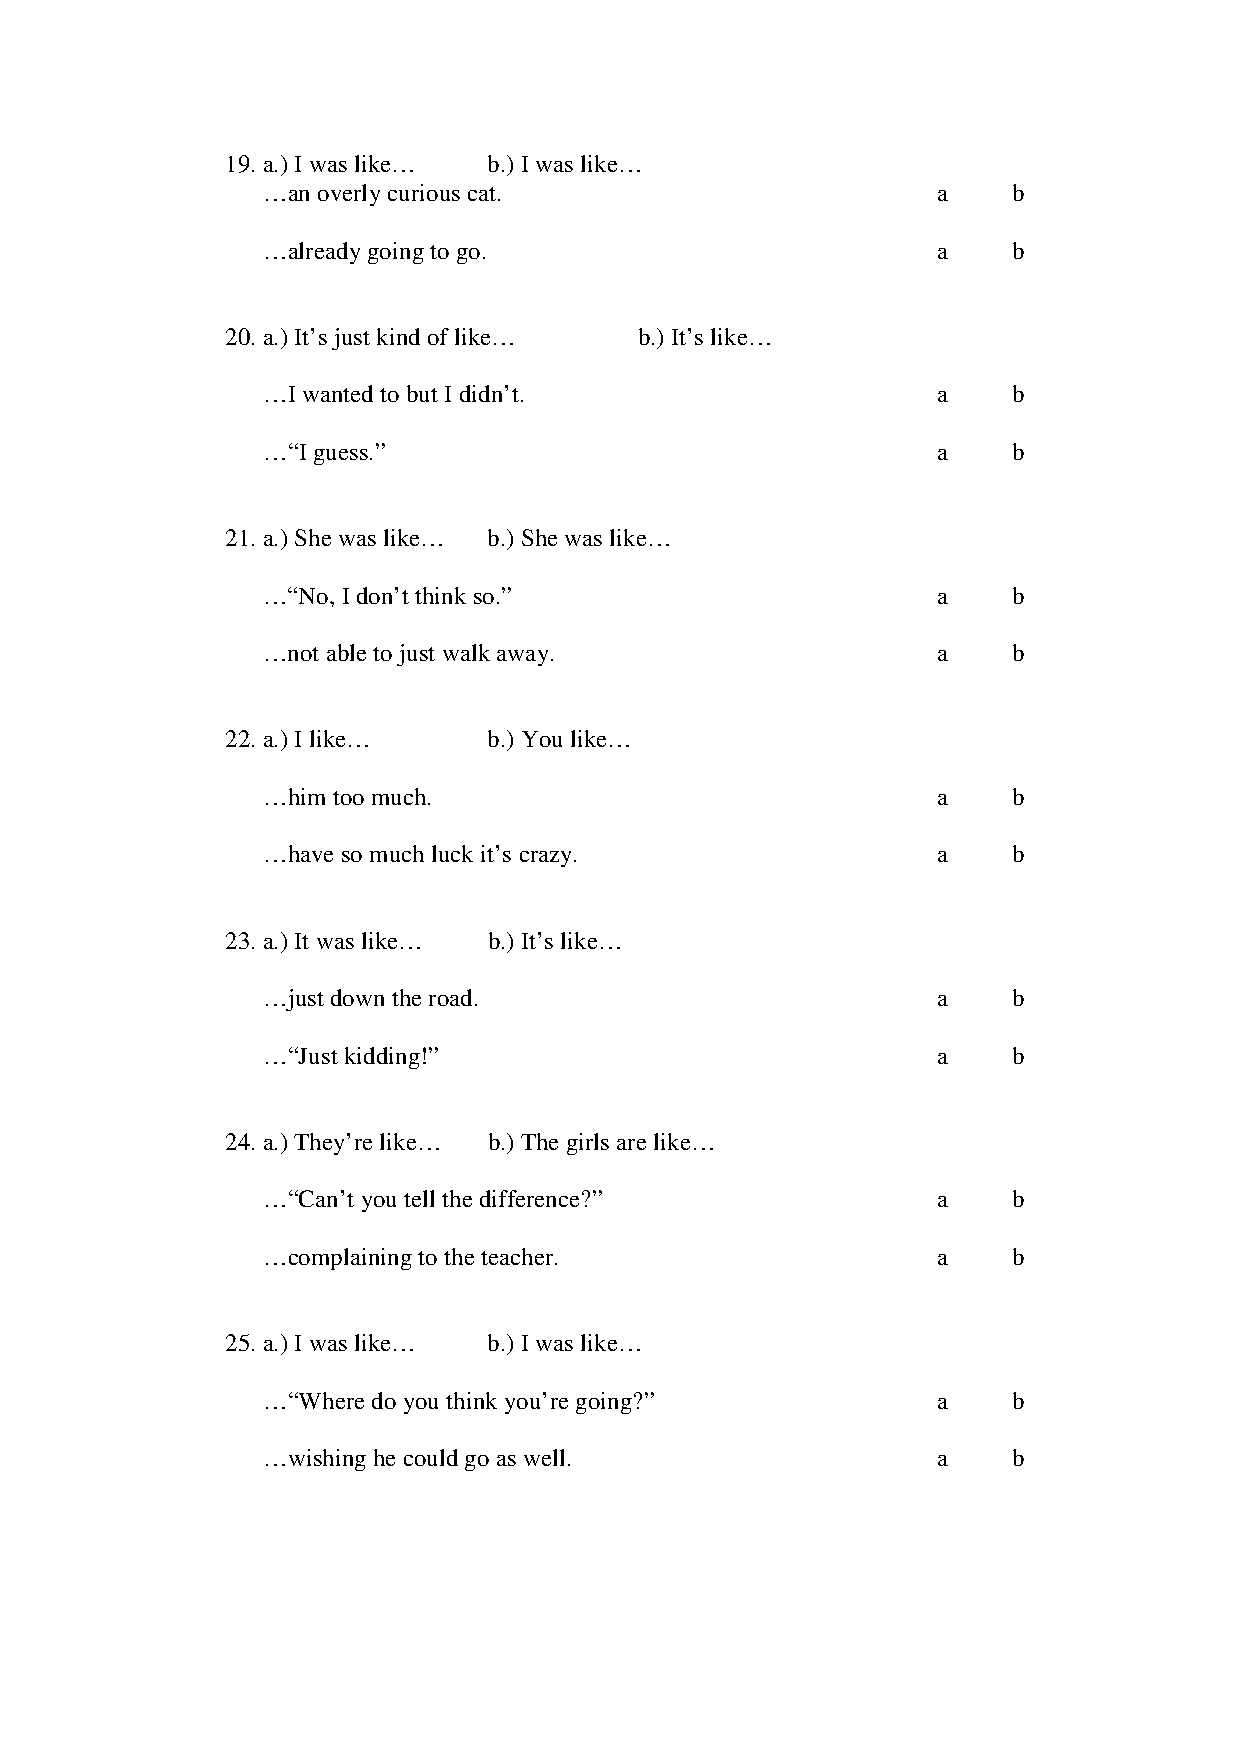
\includegraphics[width=5in]{images/Exp1page4.pdf}
		\label{x1p4}
\end{figure}

\begin{figure}[htbp]
	\centering
		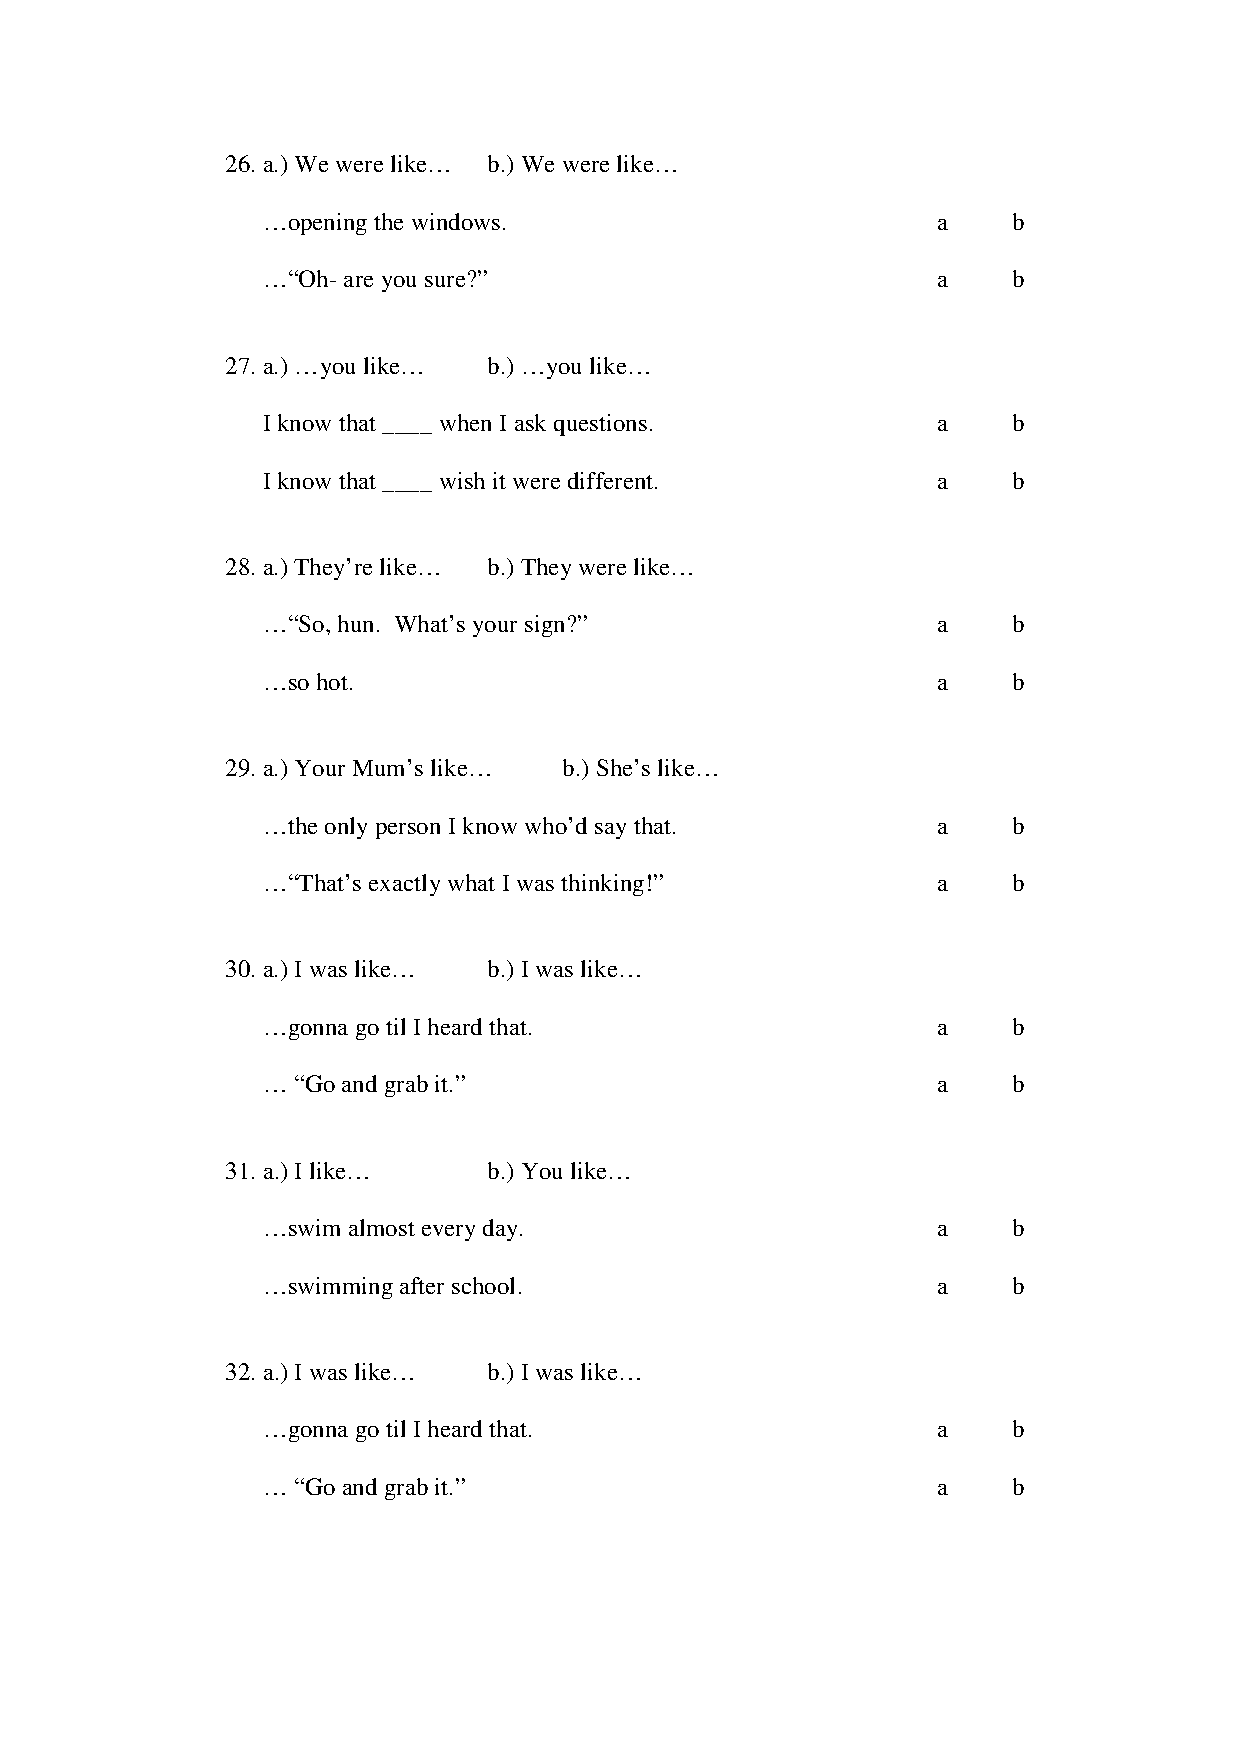
\includegraphics[width=5in]{images/Exp1page5.pdf}
		\label{x1p5}
\end{figure}

\begin{figure}[htbp]
	\centering
		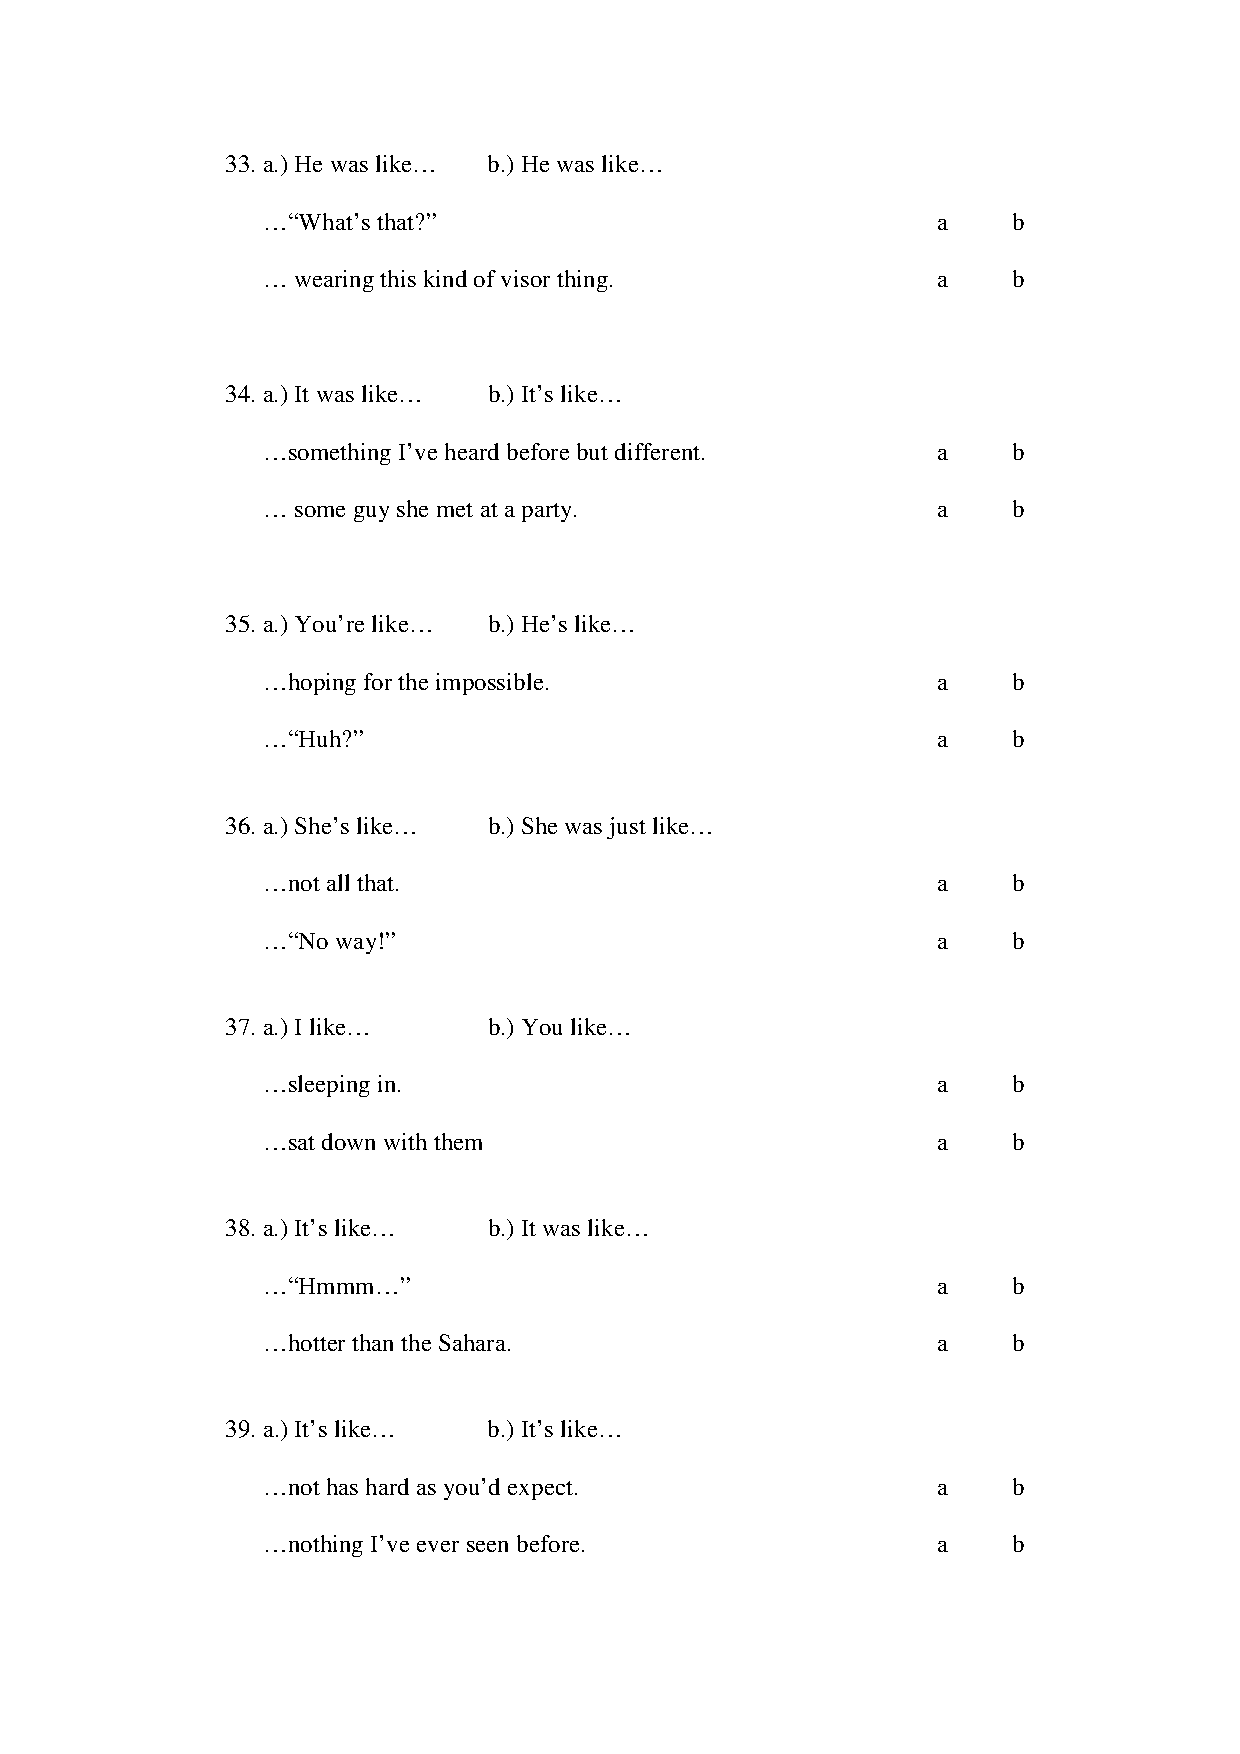
\includegraphics[width=5in]{images/Exp1page6.pdf}
	\label{x1p6}
\end{figure}

\begin{figure}[htbp]
	\centering
		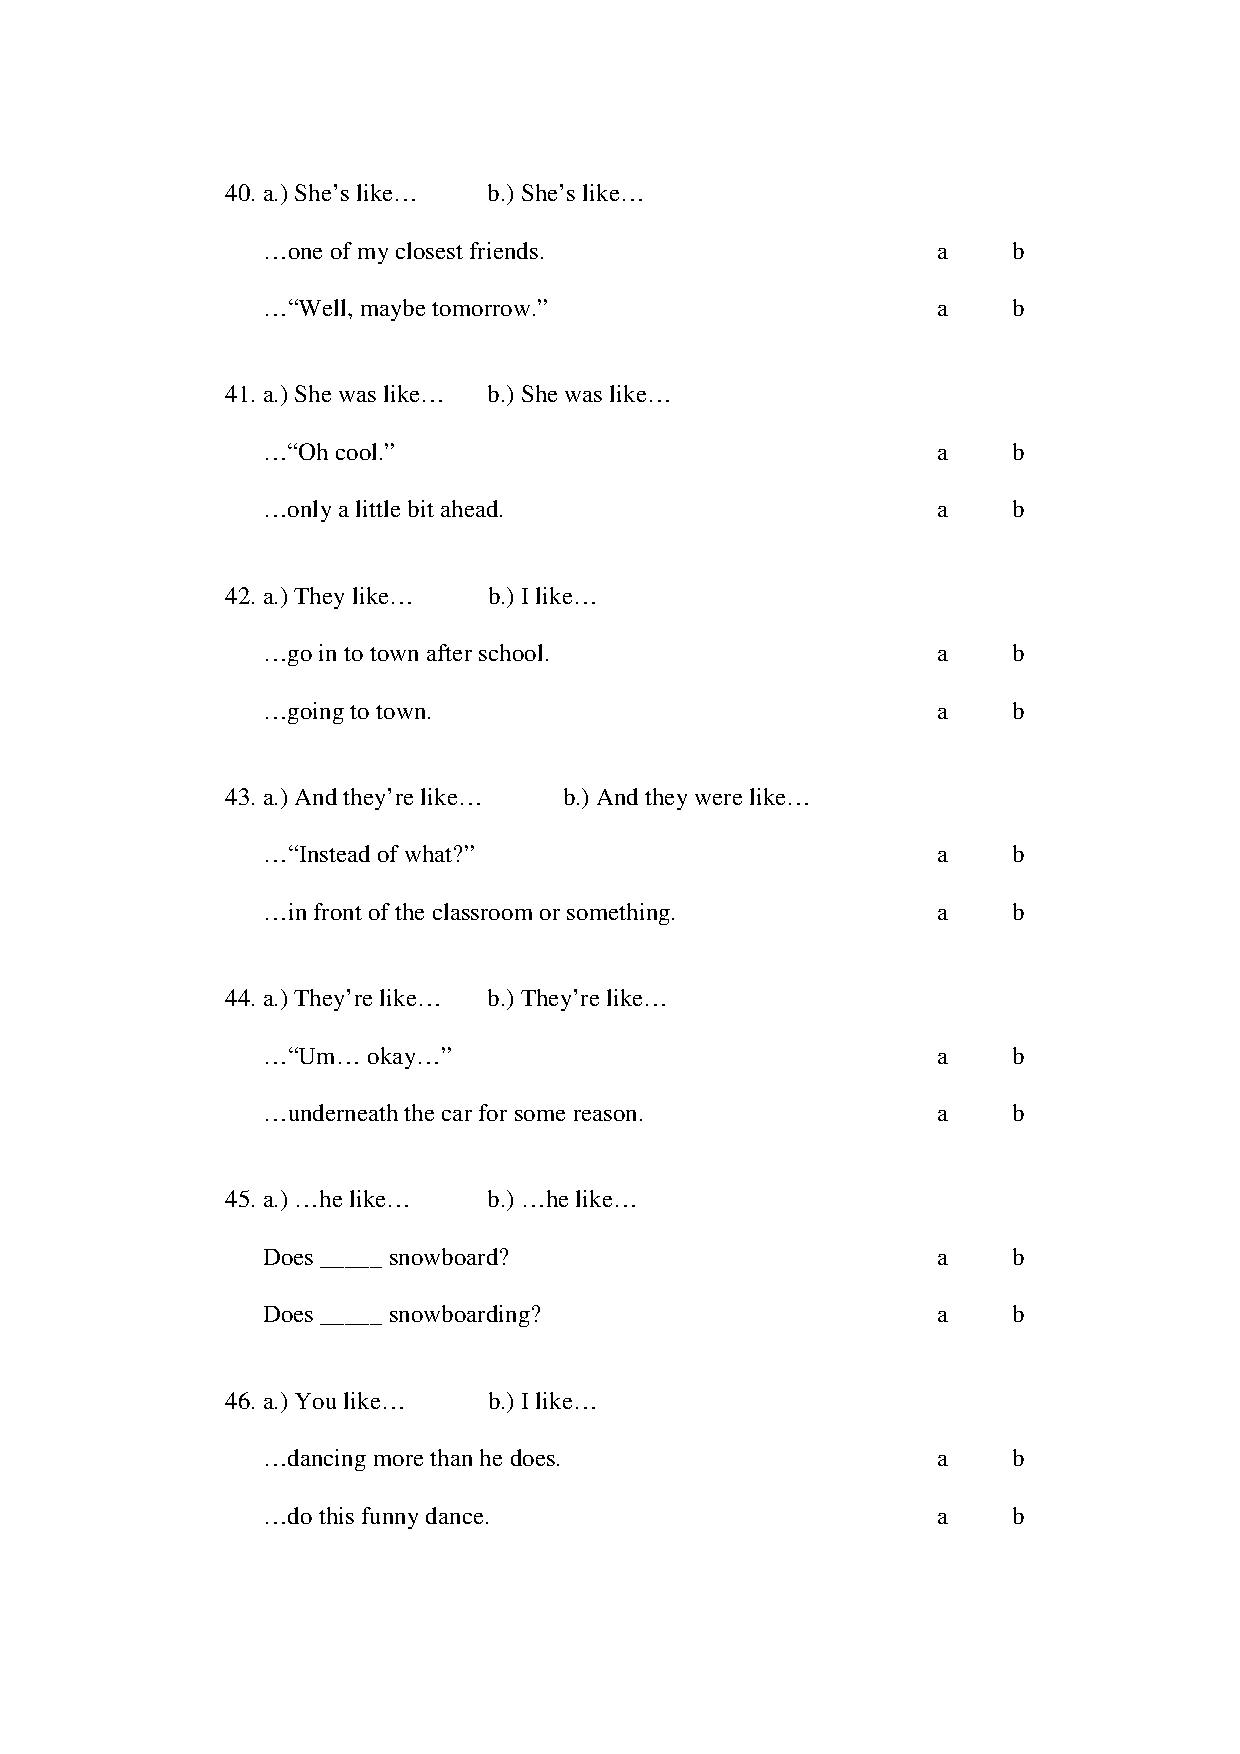
\includegraphics[width=5in]{images/Exp1page7.pdf}
	\label{x1p7}
\end{figure}

\begin{figure}[htbp]
	\centering
		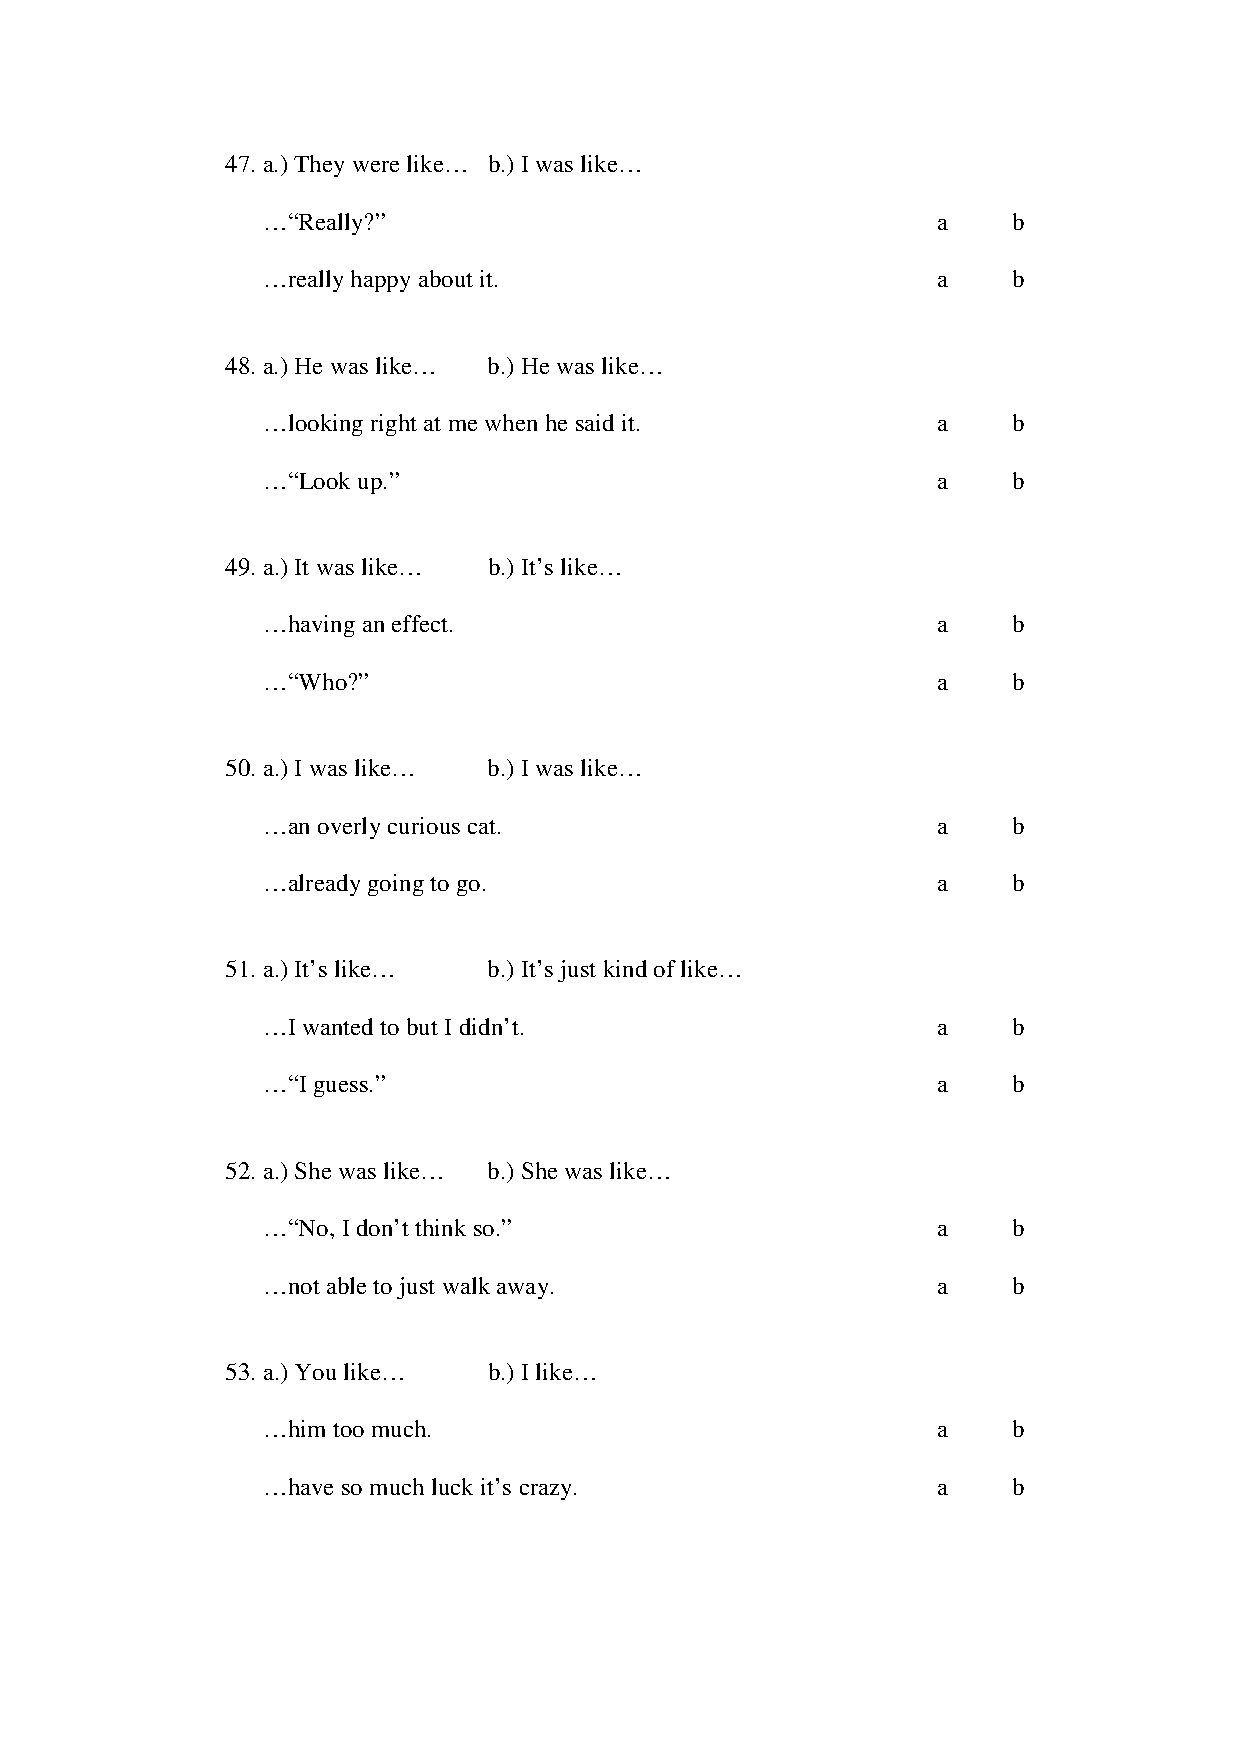
\includegraphics[width=5in]{images/Exp1page8.pdf}
		\label{x1p8}
\end{figure}

\begin{figure}[htbp]
	\centering
		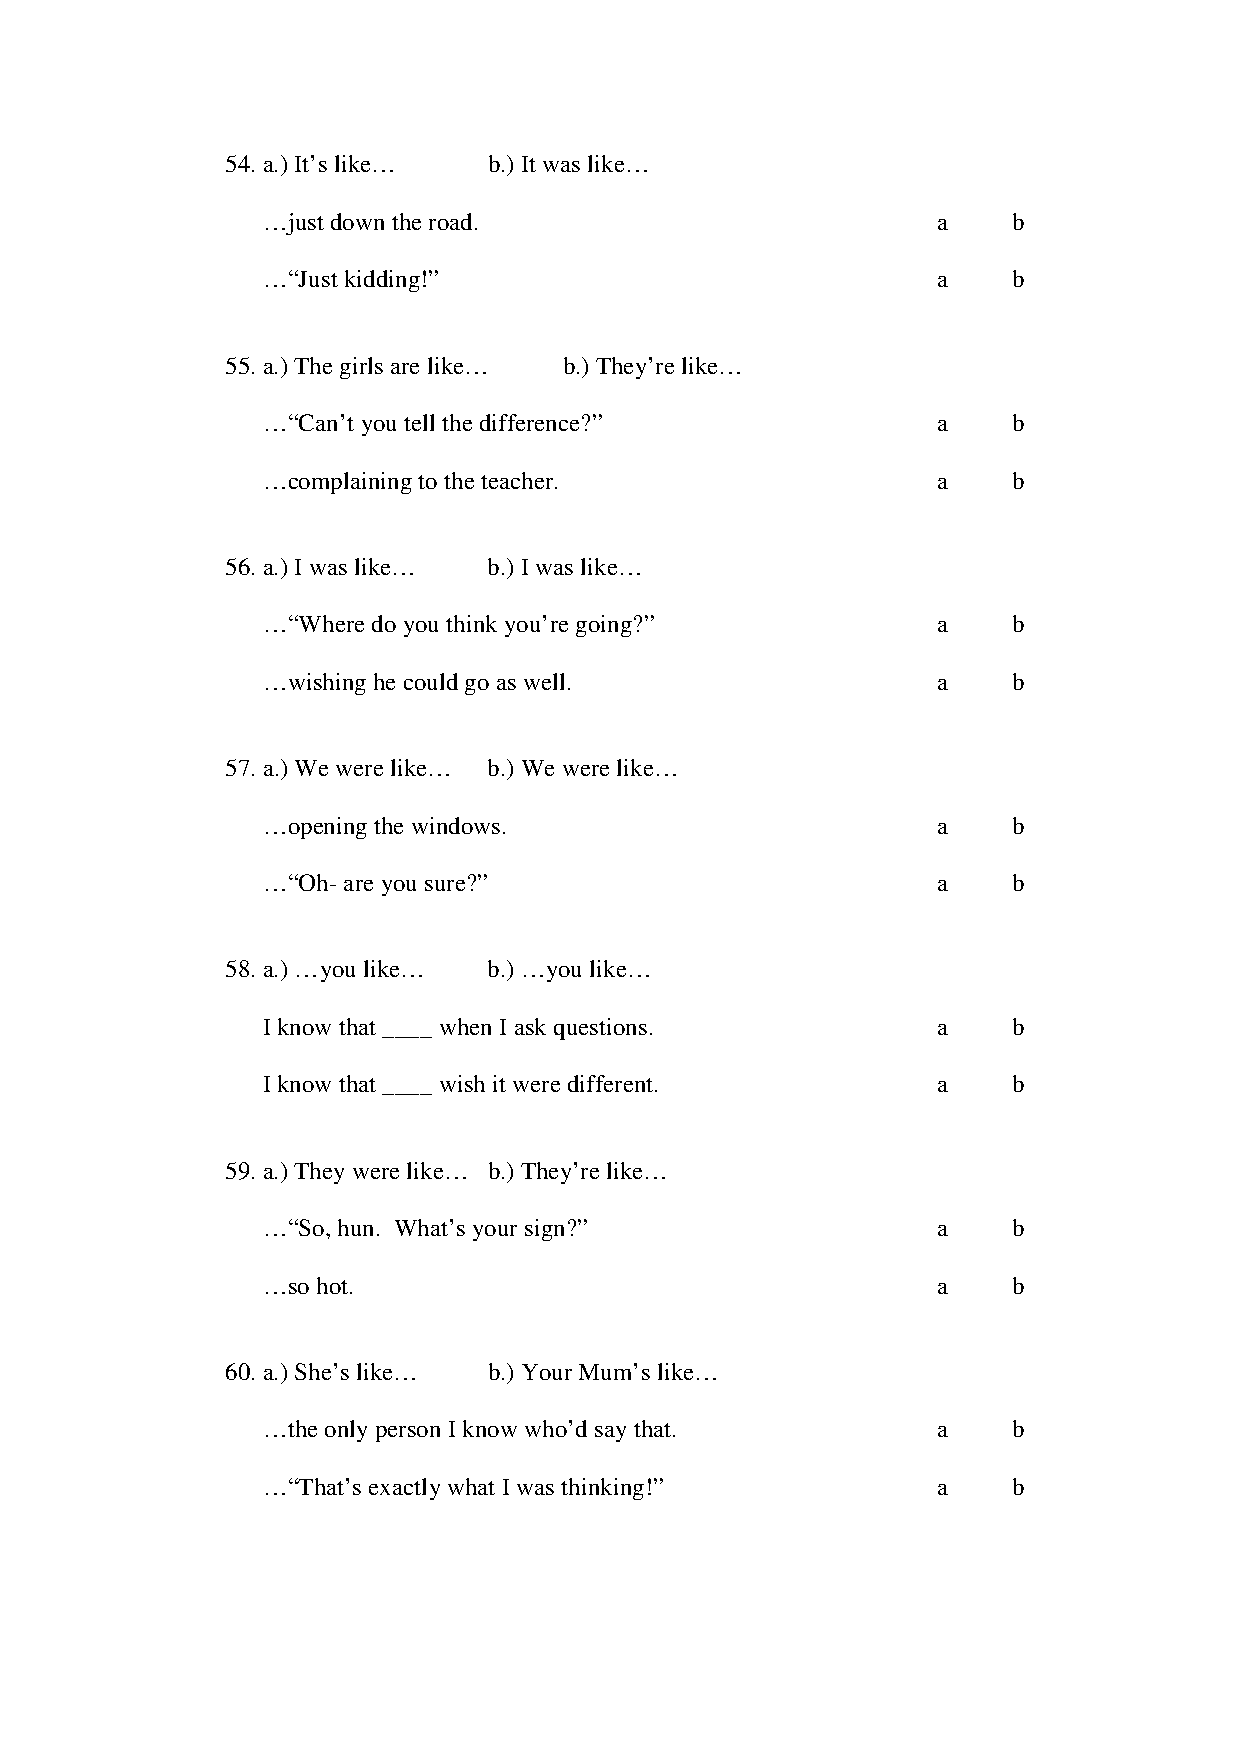
\includegraphics[width=5in]{images/Exp1page9.pdf}
		\label{x1p9}
\end{figure}

\begin{figure}[htbp]
	\centering
		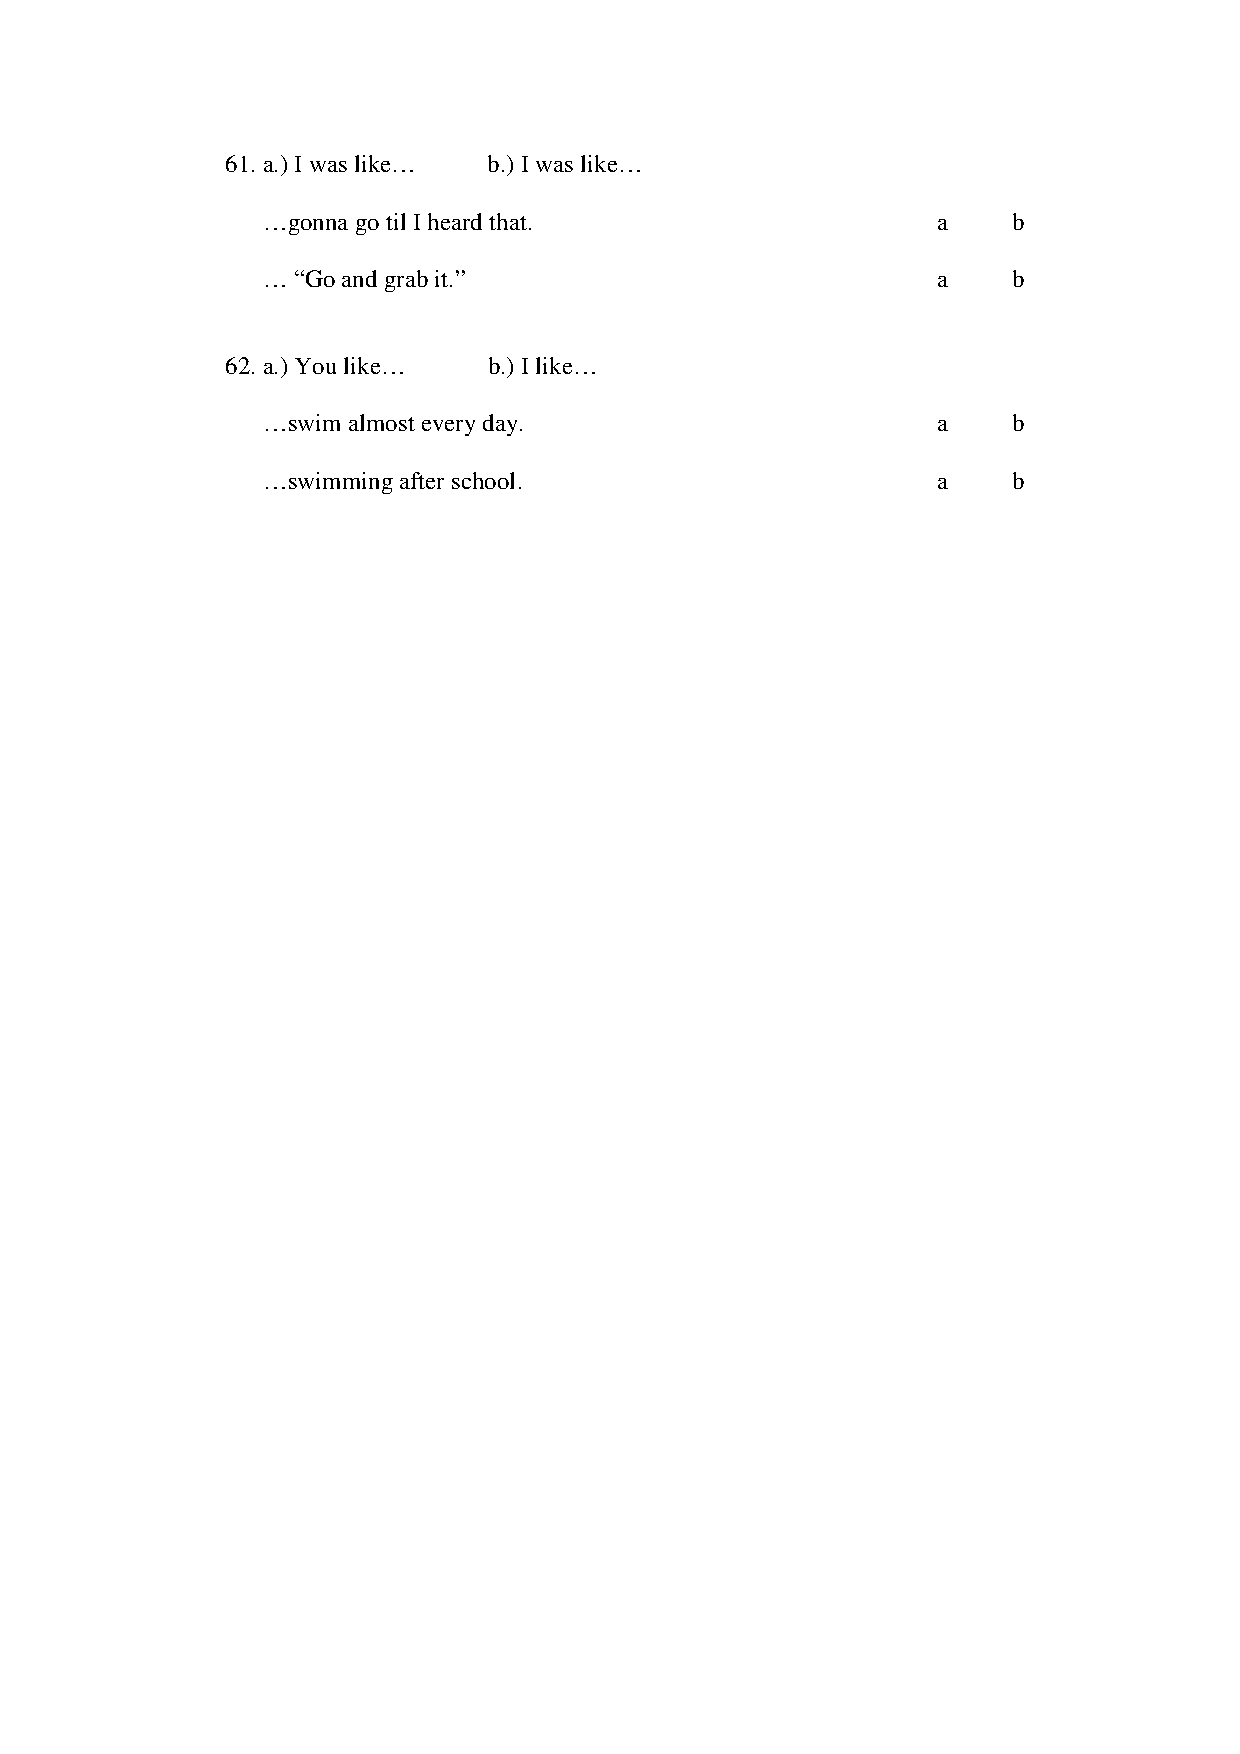
\includegraphics[width=5in]{images/Exp1page10.pdf}
		\label{x1p10}
\end{figure}


\clearpage
\begin{figure}[htbp]
	\centering
		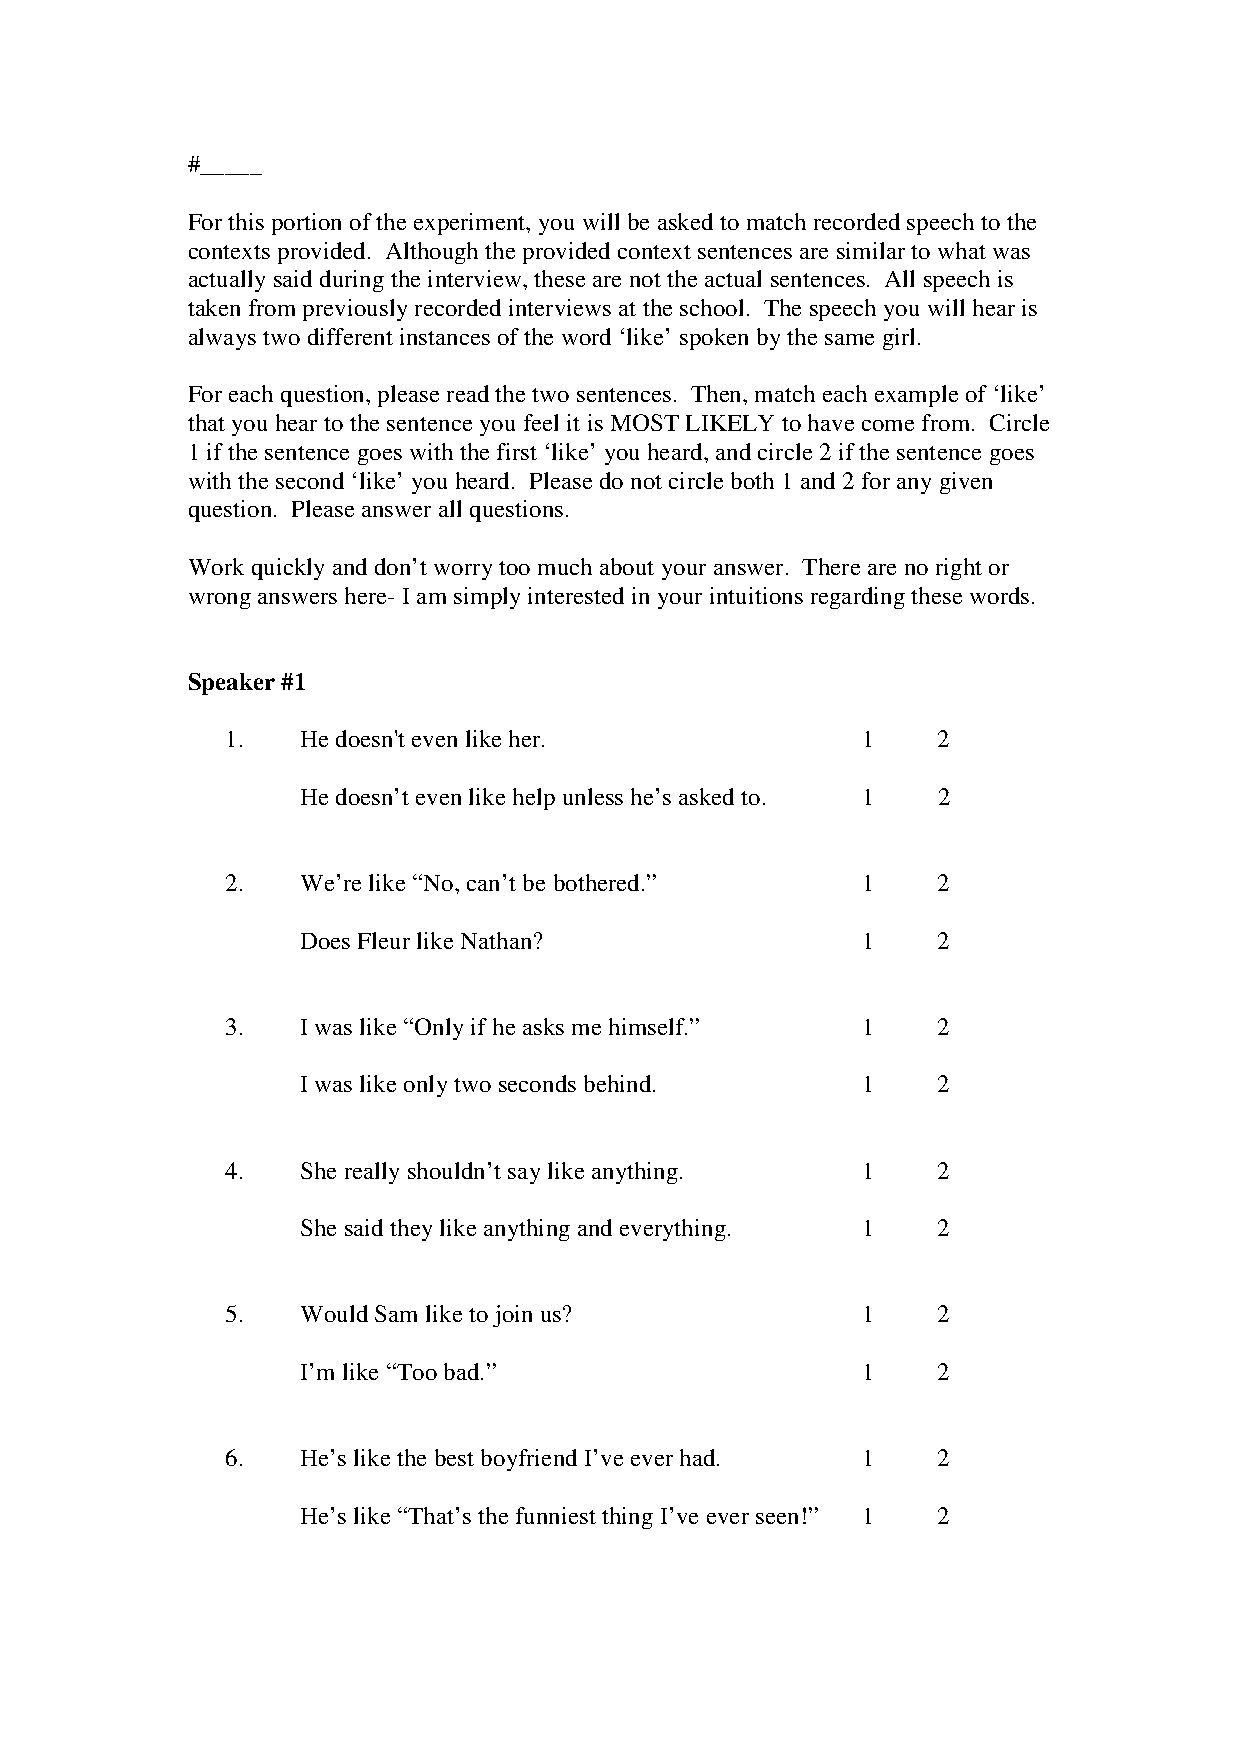
\includegraphics[width=5in]{images/Exp2page1.pdf}
		\caption{Answersheet for Experiment 2}
		\label{x2p1}
\end{figure}

\begin{figure}
	\centering
		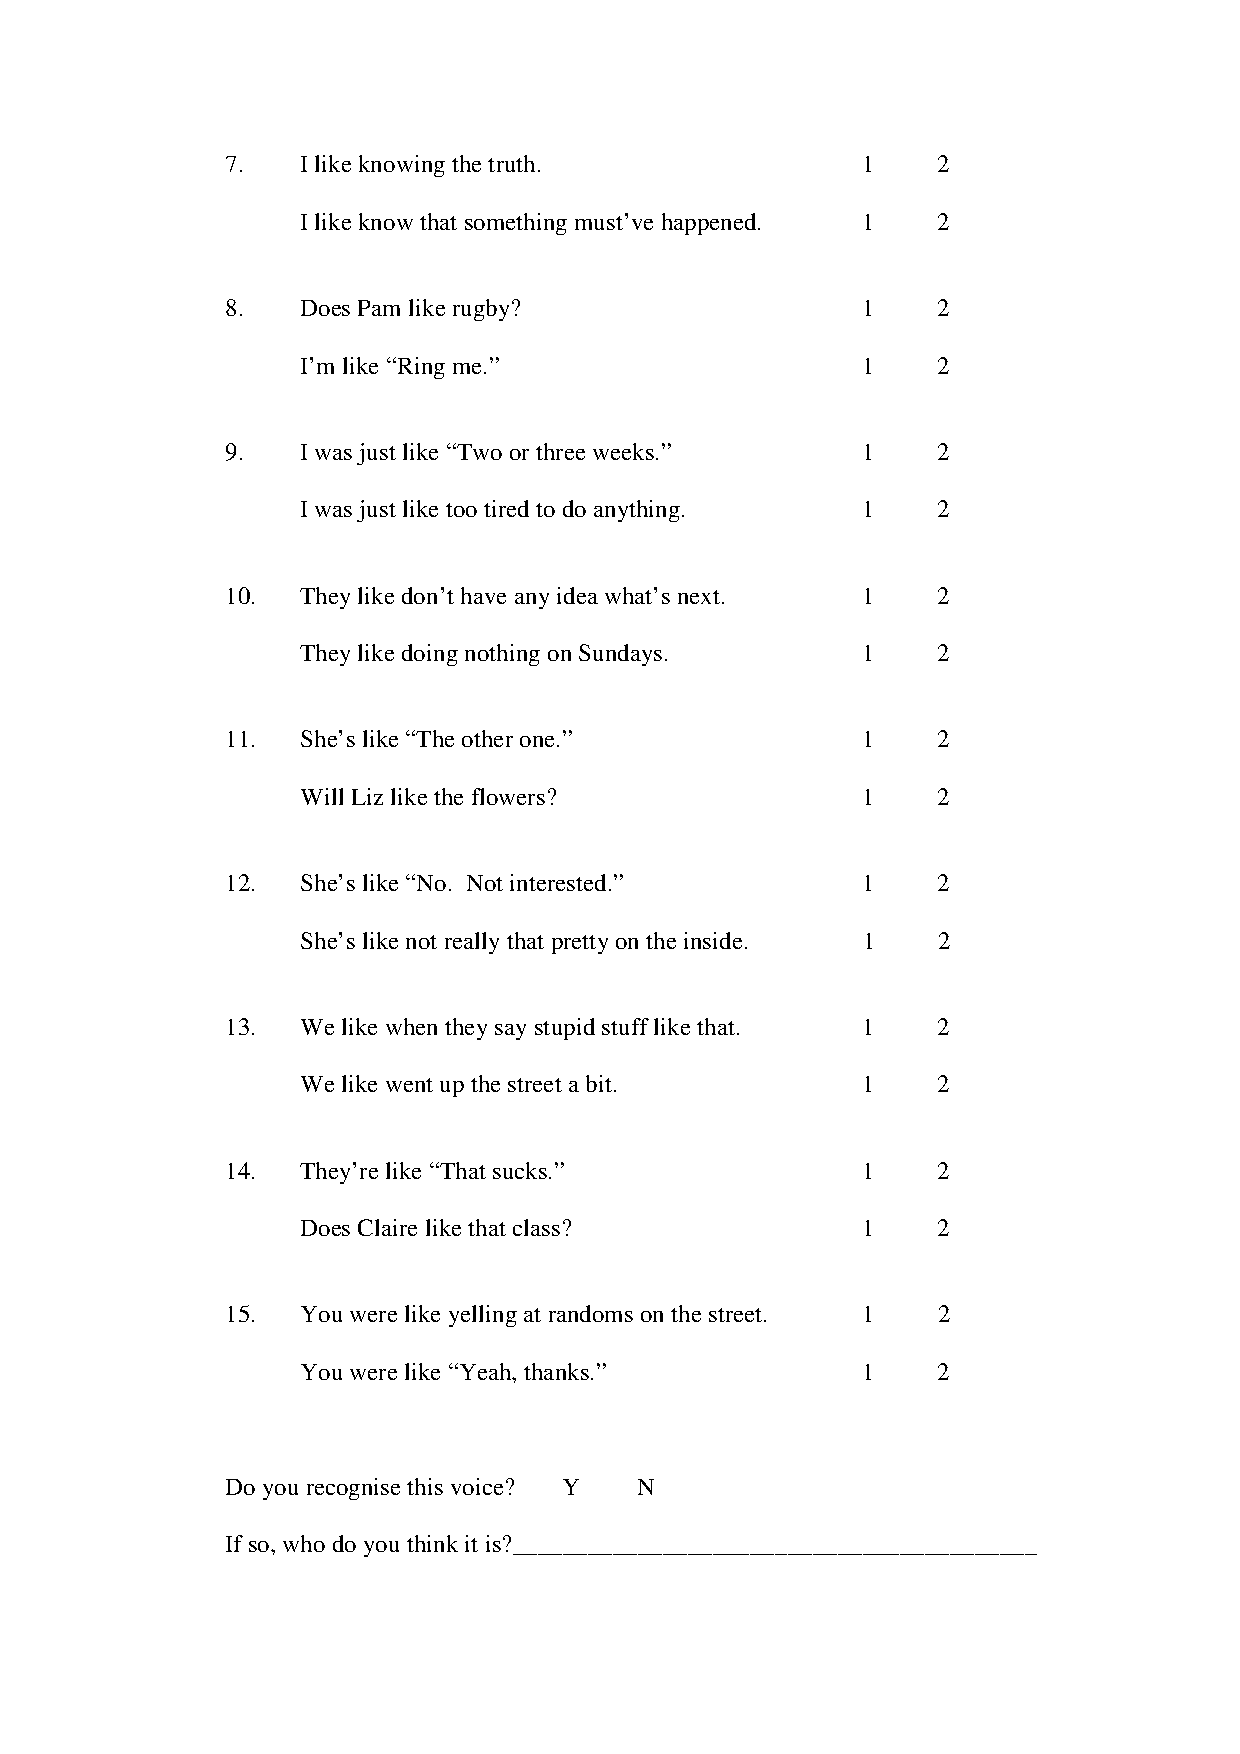
\includegraphics[width=5in]{images/Exp2page2.pdf}
			\label{x2p2}
\end{figure}

\begin{figure}
	\centering
		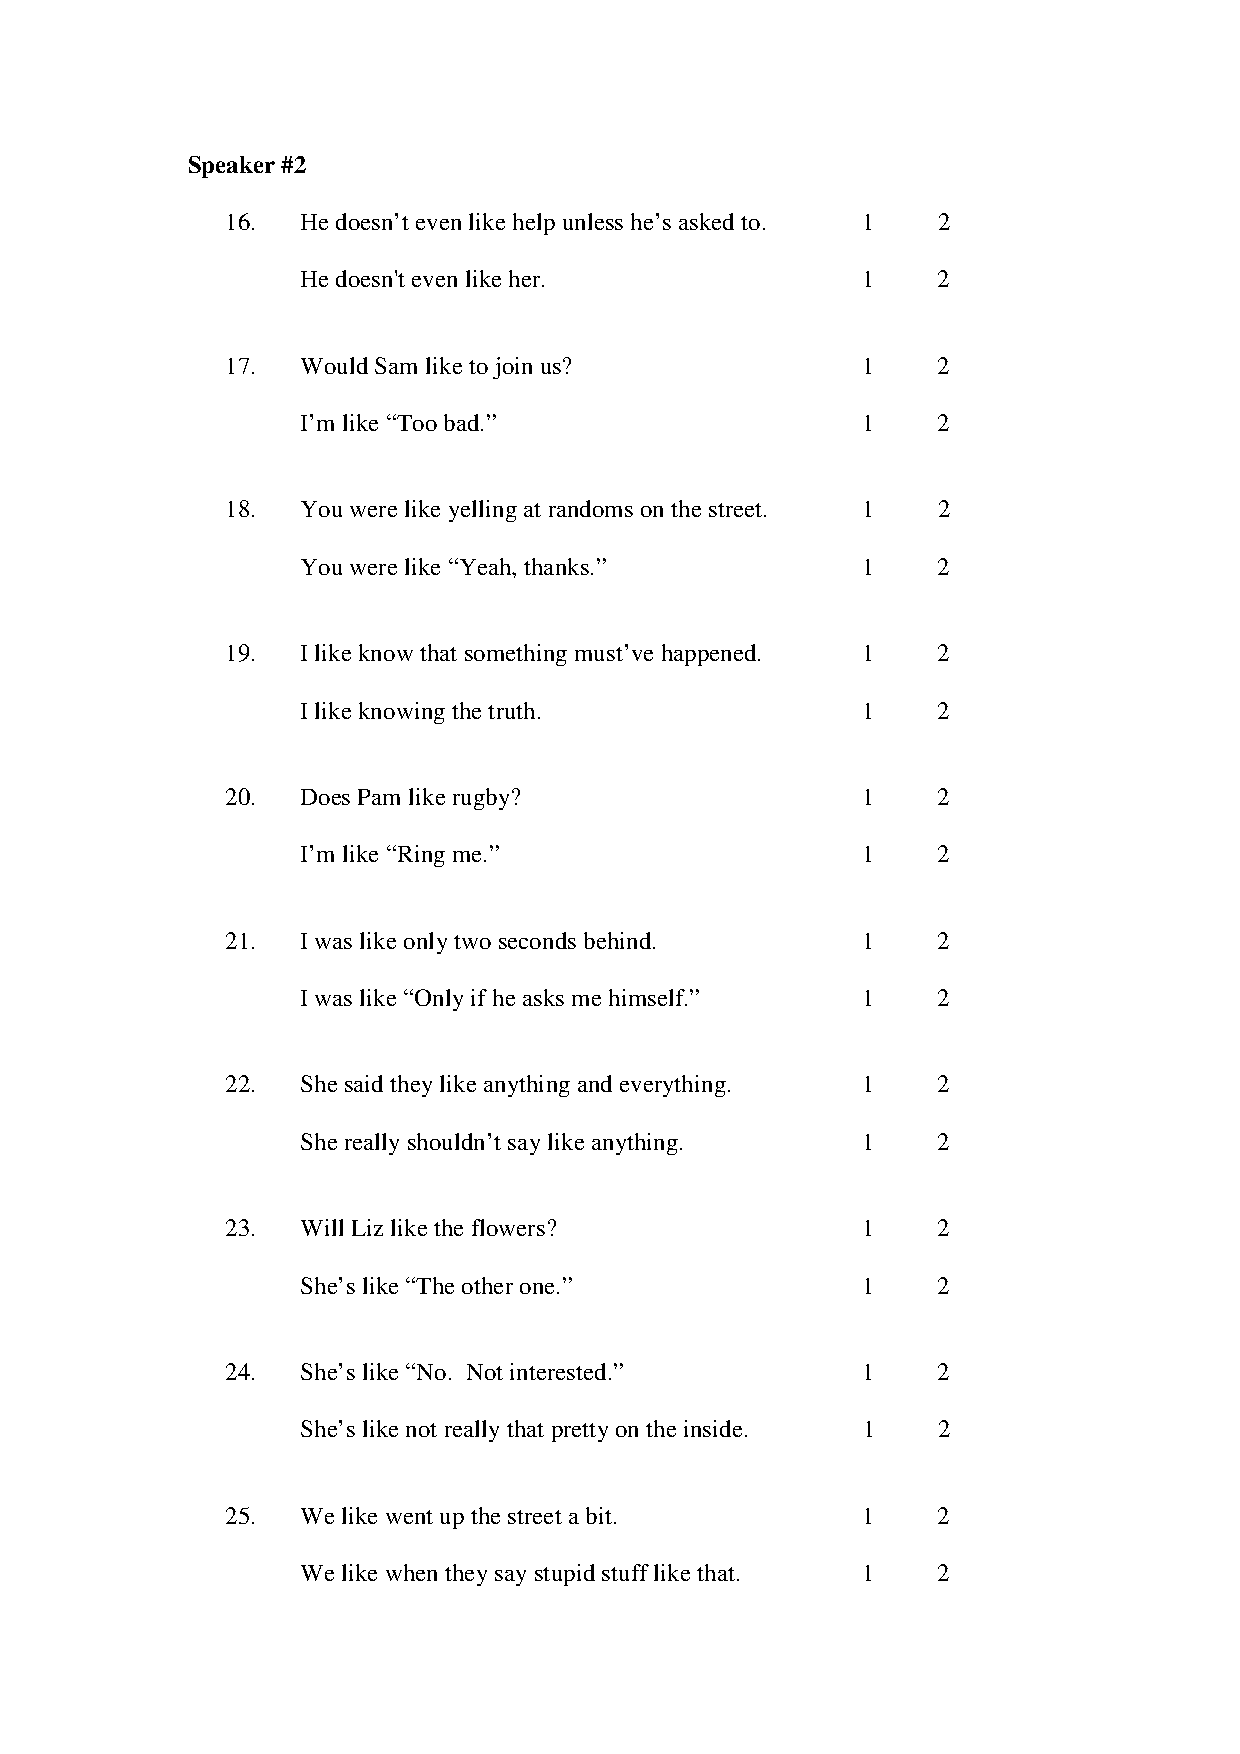
\includegraphics[width=5in]{images/Exp2page3.pdf}
			\label{x2p3}
\end{figure}

\begin{figure}
	\centering
		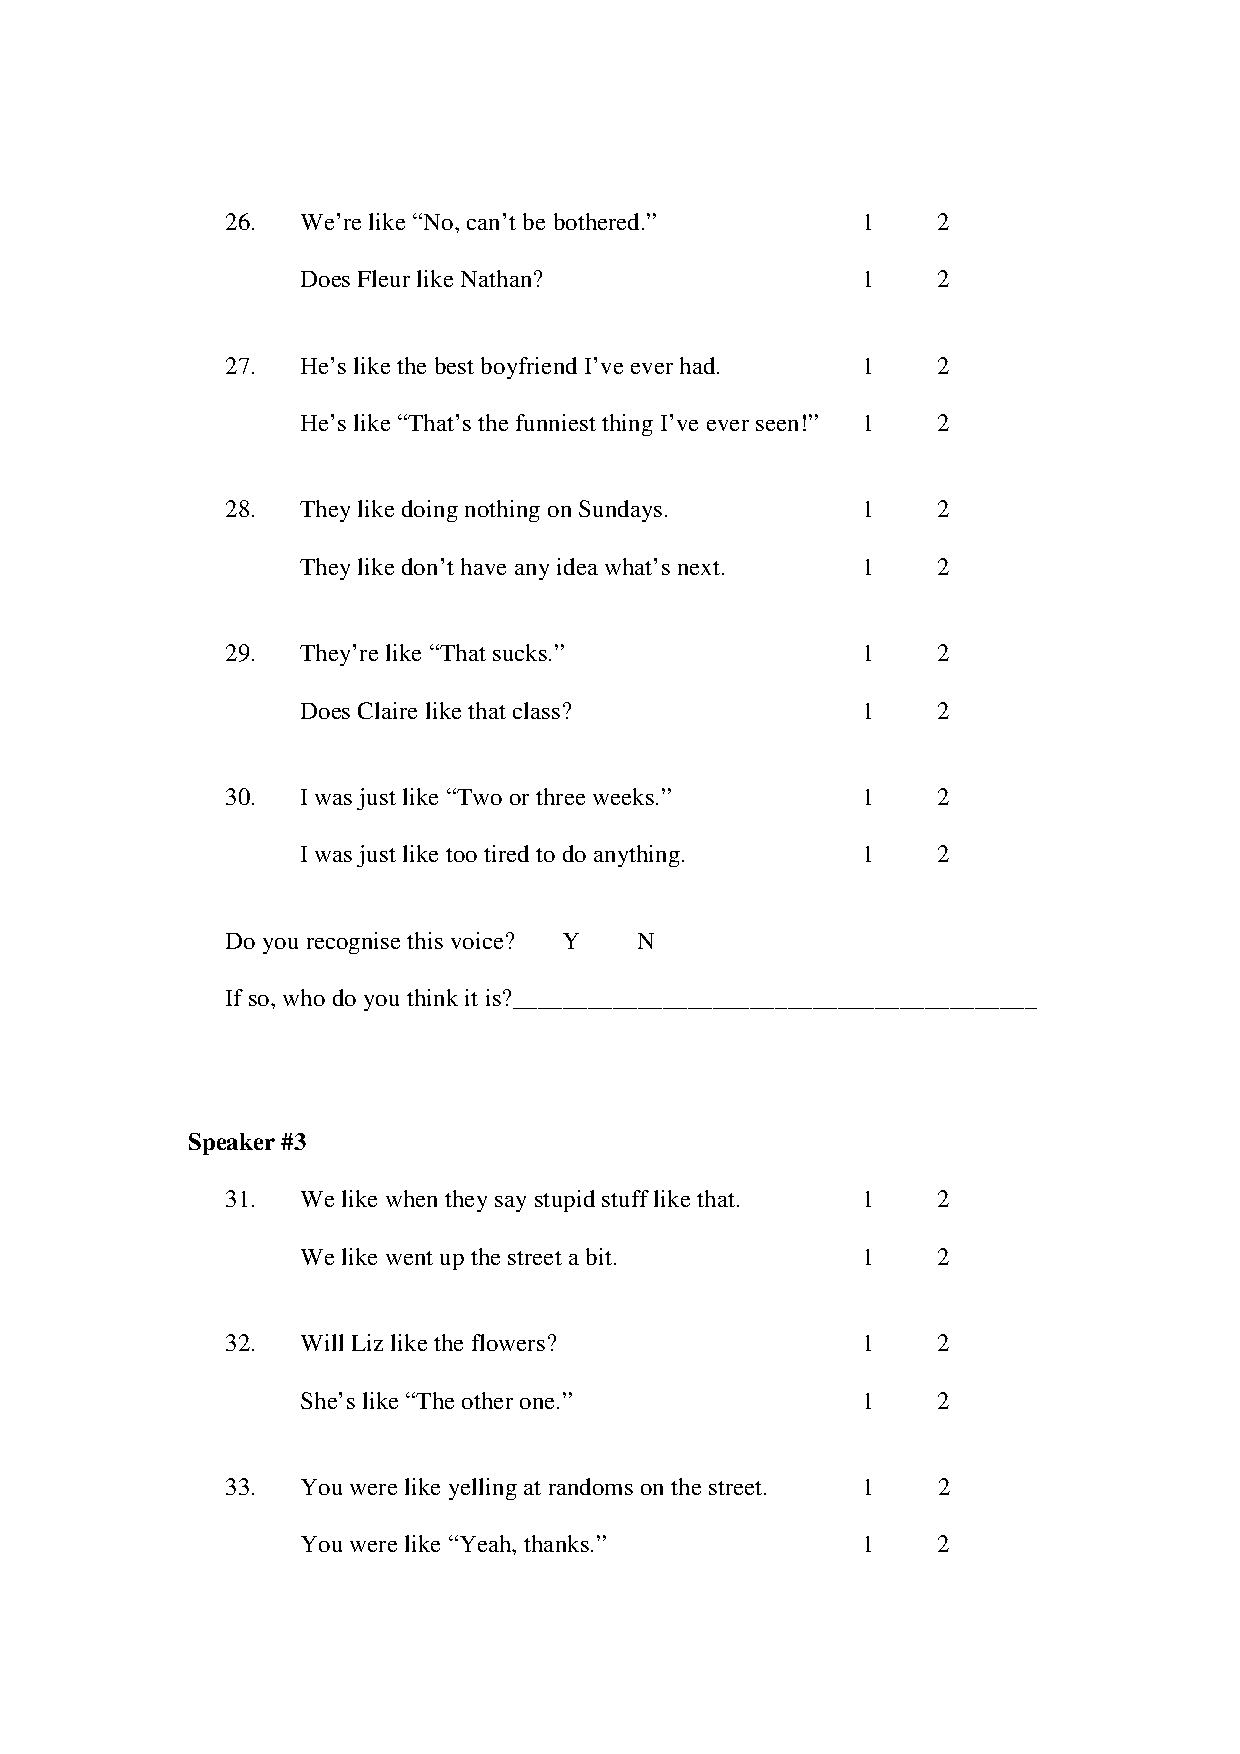
\includegraphics[width=5in]{images/Exp2page4.pdf}
			\label{x2p4}
\end{figure}

\begin{figure}
	\centering
		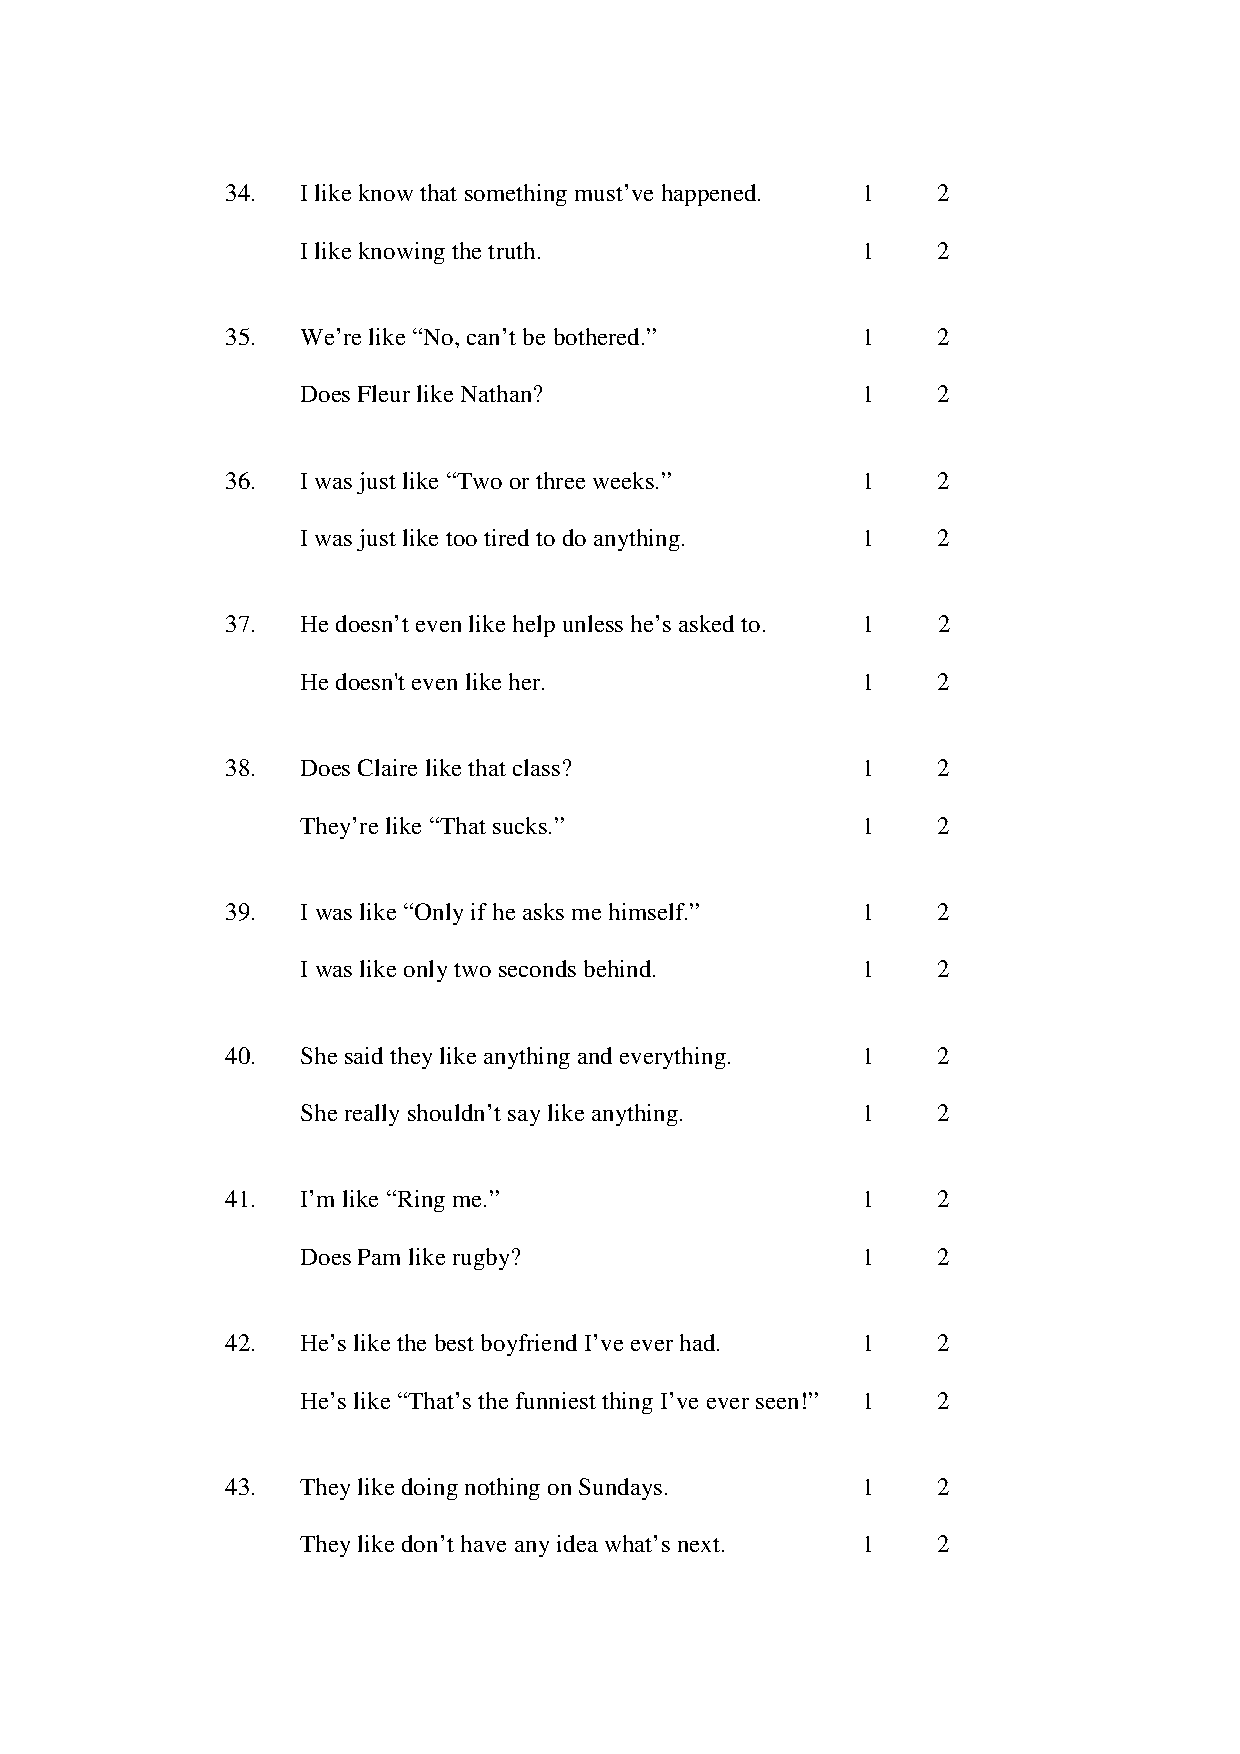
\includegraphics[width=5in]{images/Exp2page5.pdf}
			\label{x2p5}
\end{figure}

\begin{figure}
	\centering
		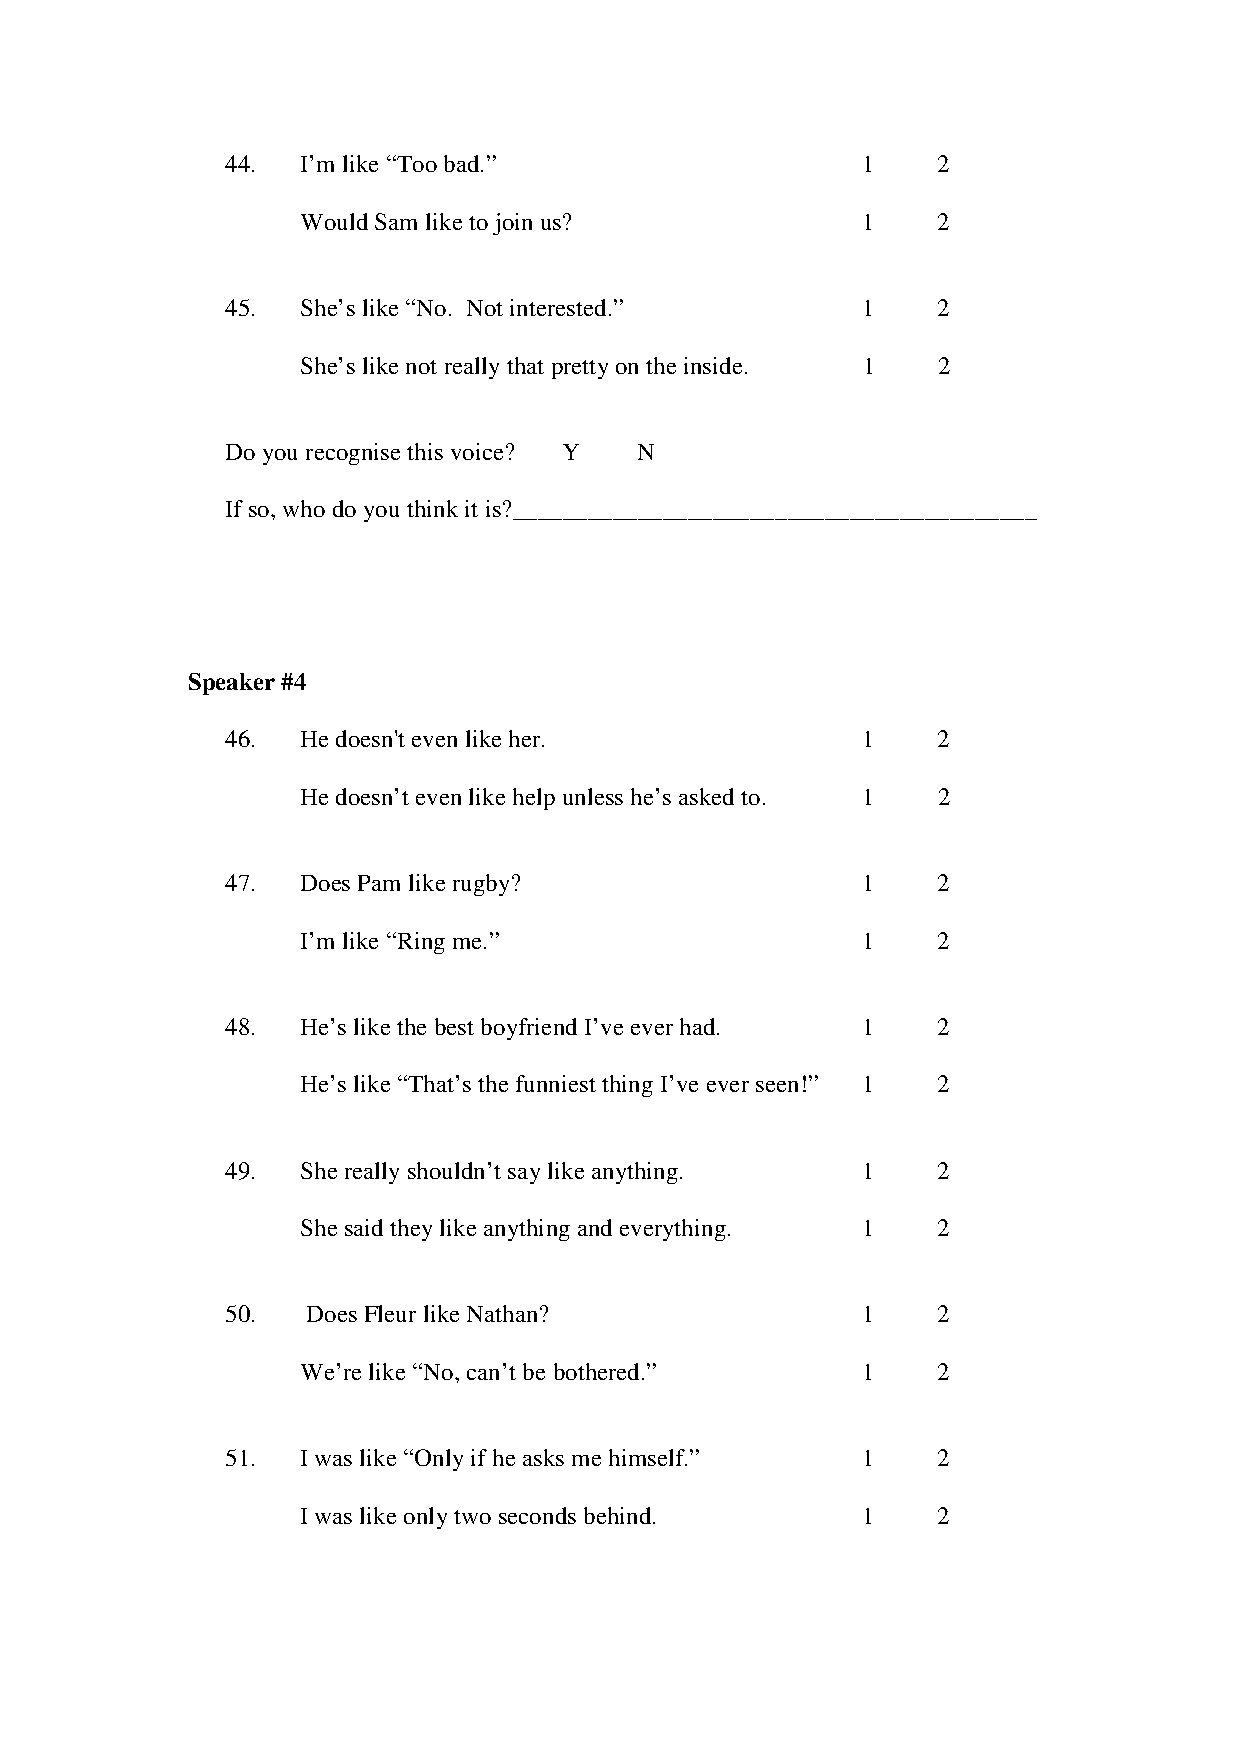
\includegraphics[width=5in]{images/Exp2page6.pdf}
			\label{x2p6}
\end{figure}

\begin{figure}
	\centering
		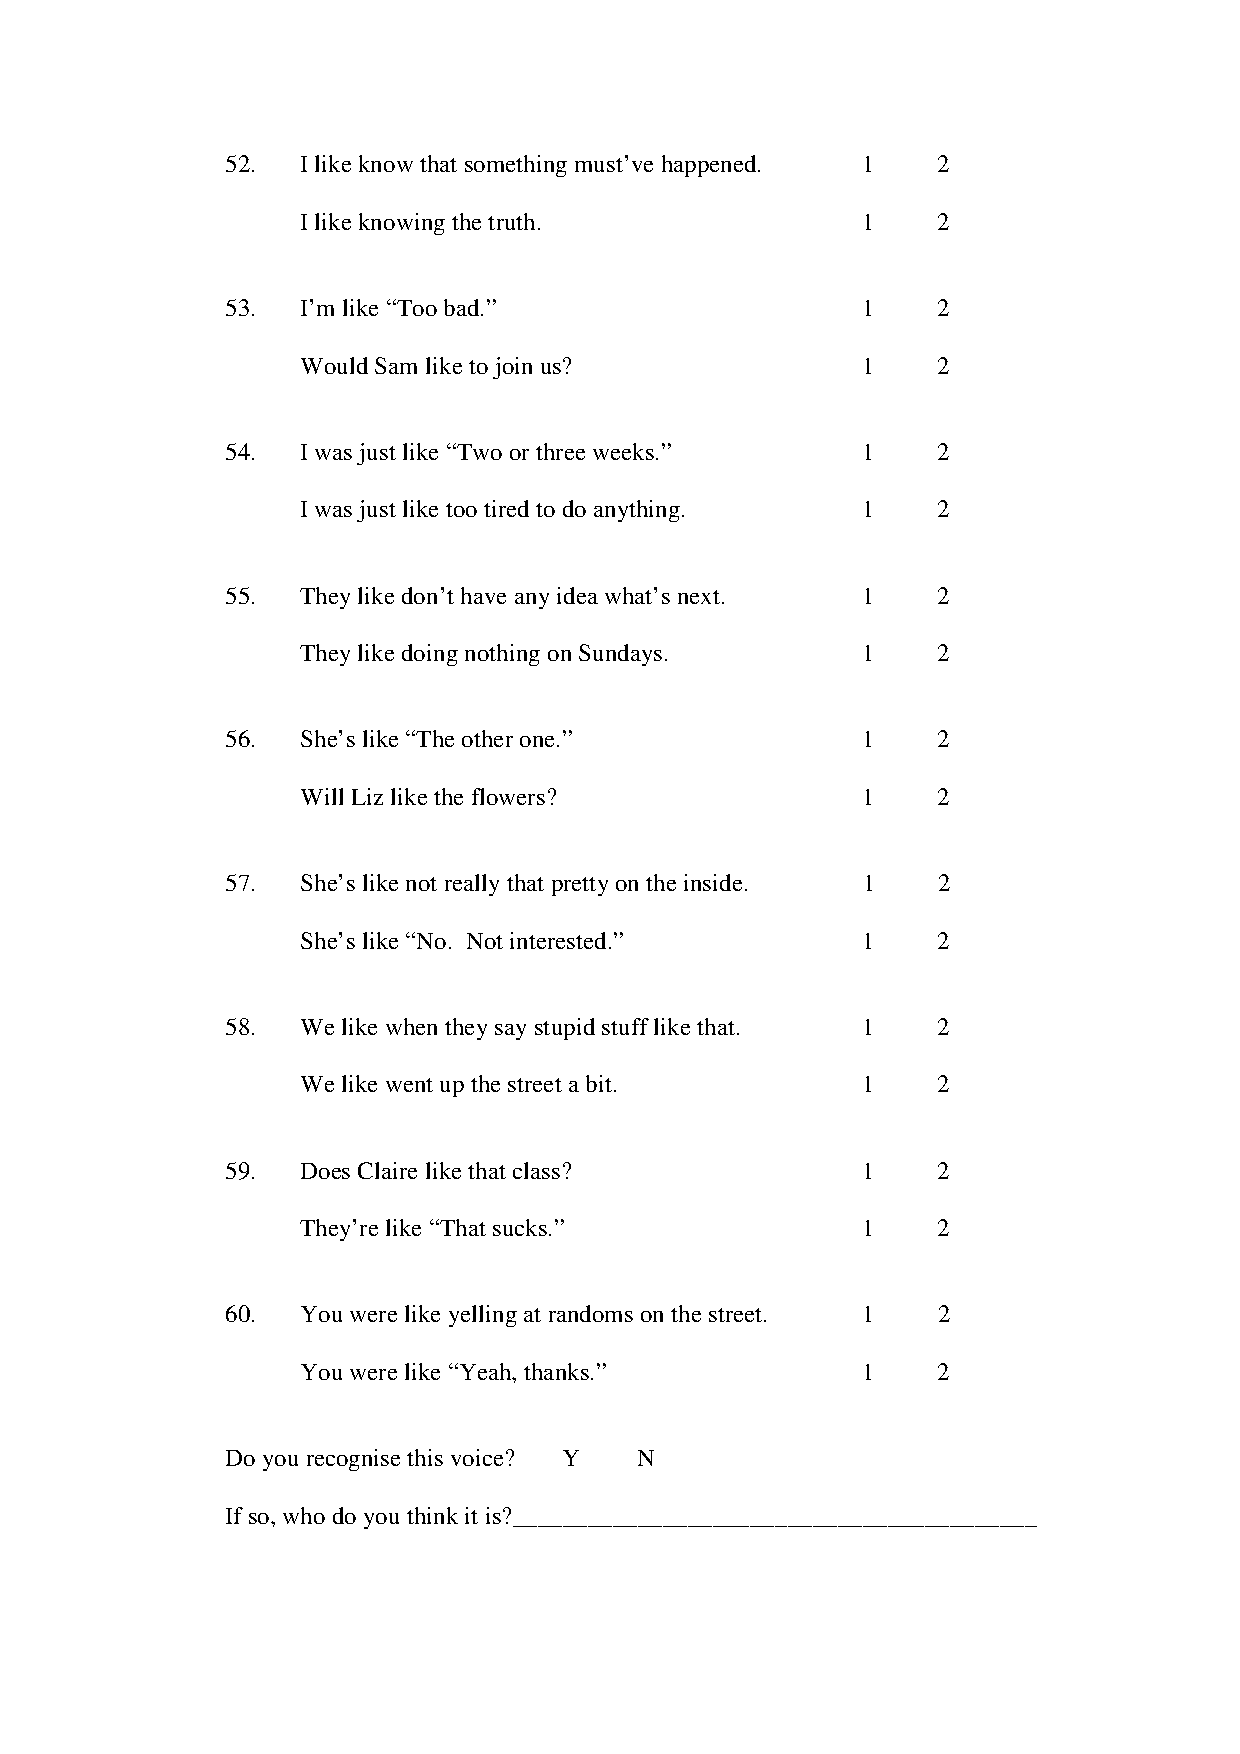
\includegraphics[width=5in]{images/Exp2page7.pdf}
			\label{x2p7}
\end{figure}



\begin{figure}
	\centering
		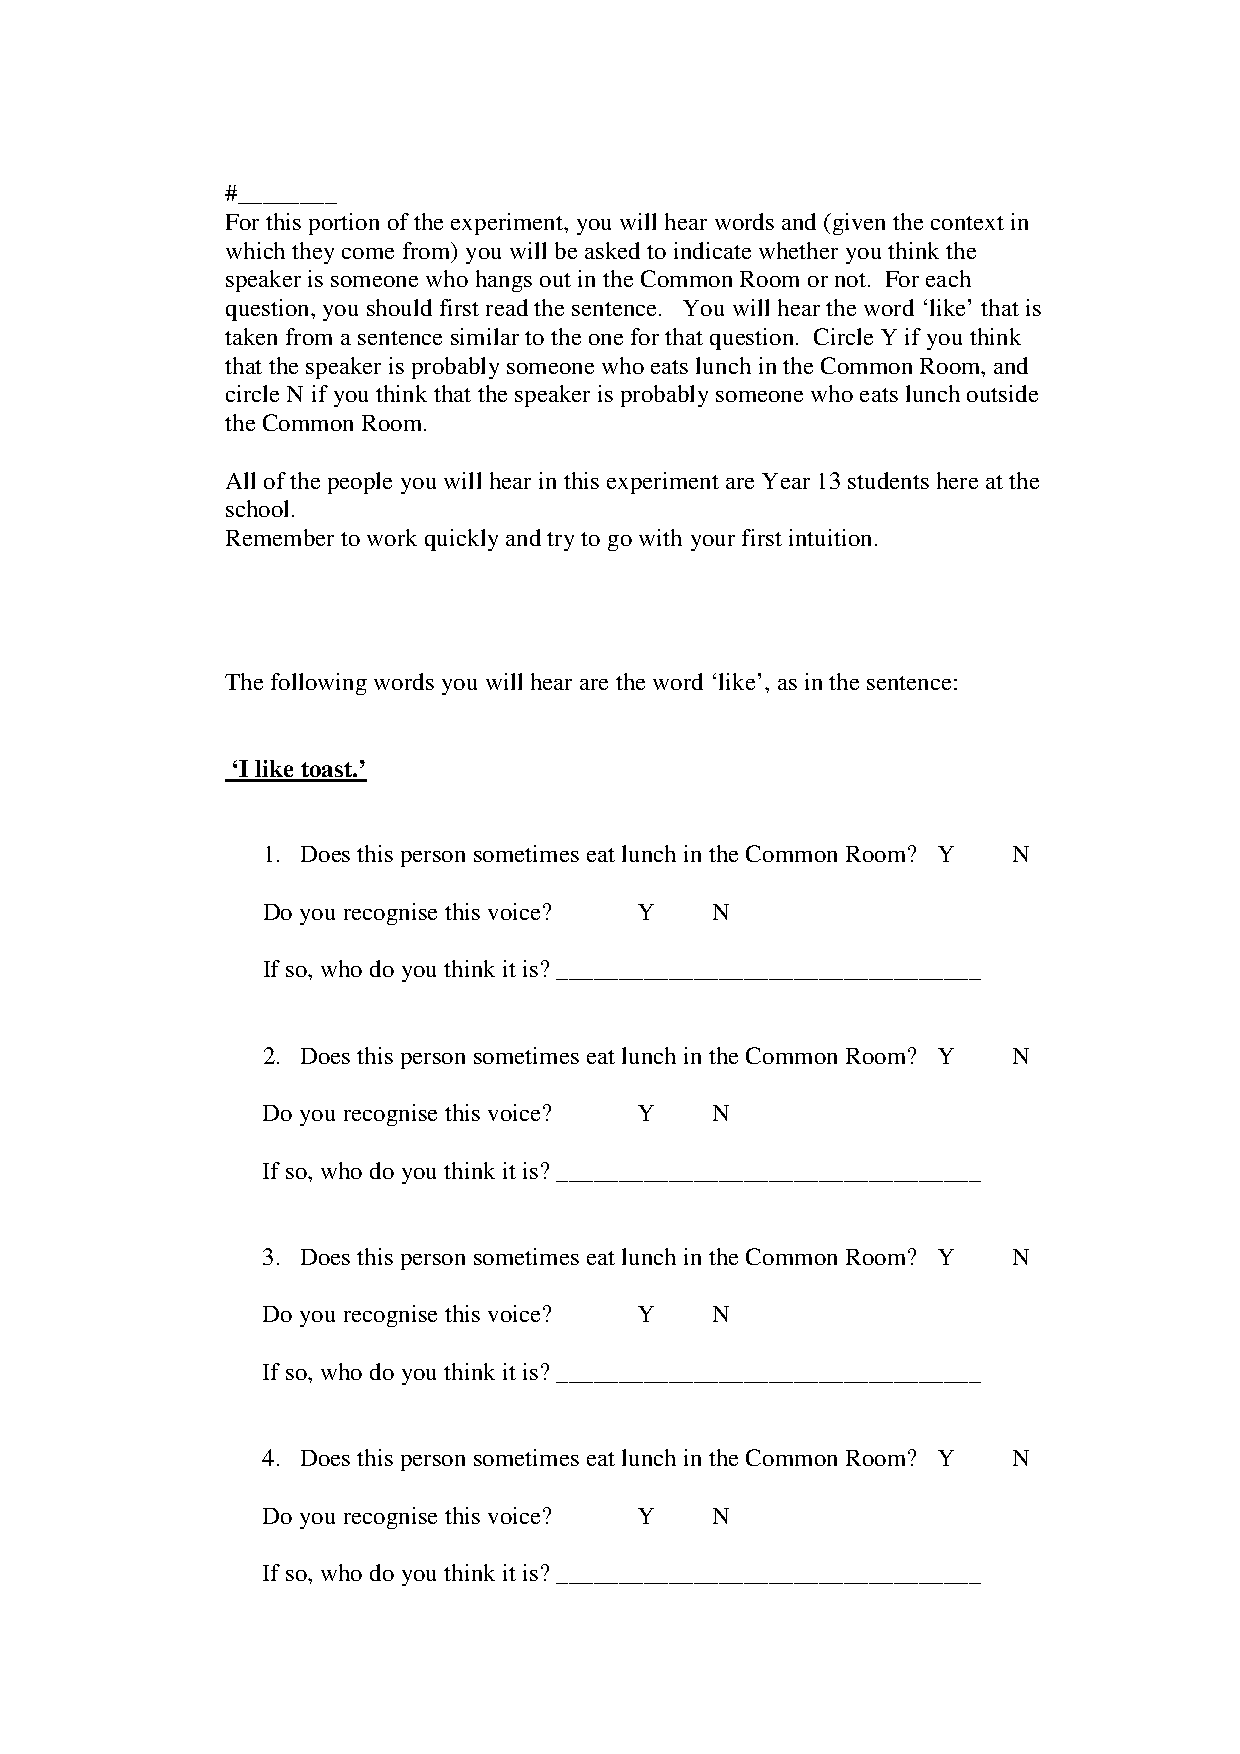
\includegraphics[width=5in]{images/Exp3page1.pdf}
		\caption{Answersheet for Experiment 3}
			\label{x3p1}
\end{figure}

\begin{figure}
	\centering
		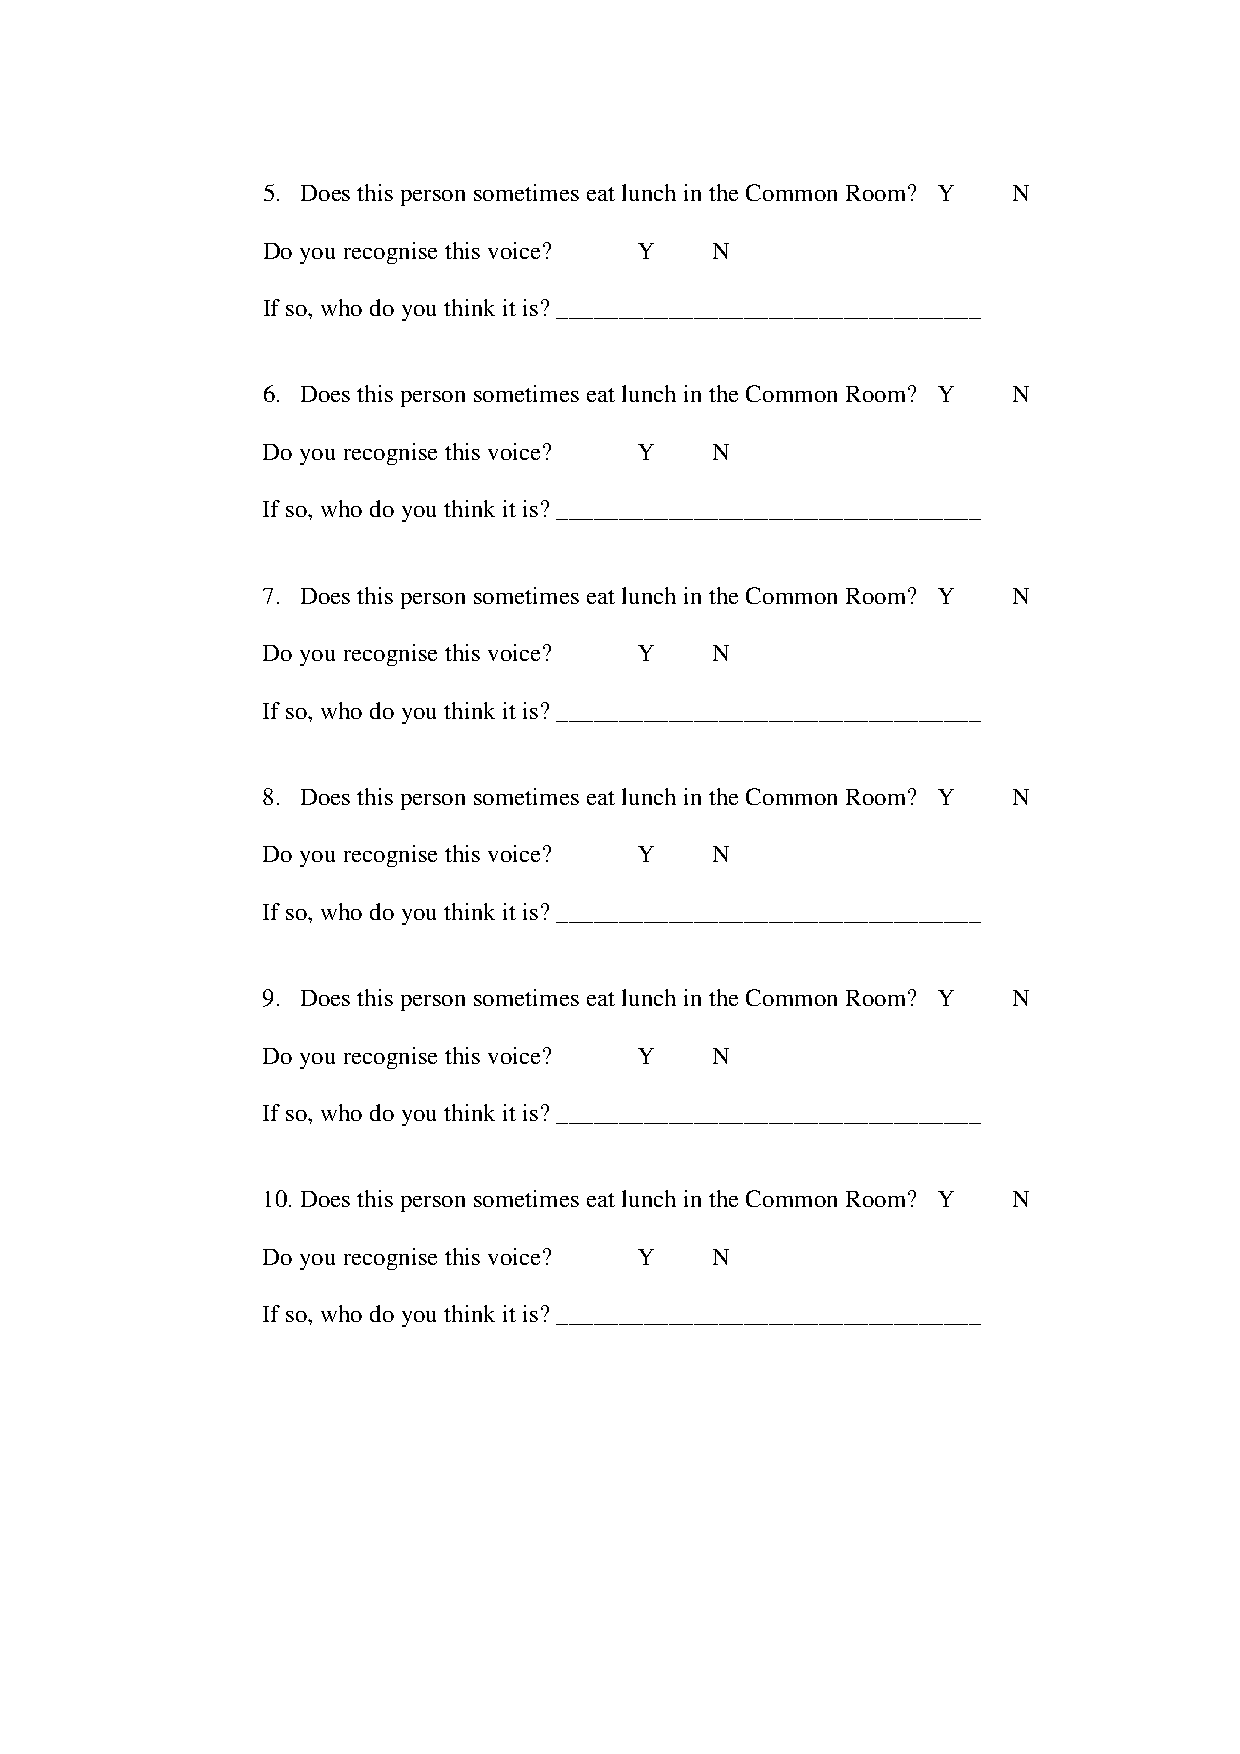
\includegraphics[width=5in]{images/Exp3page2.pdf}
		\label{x3p2}
\end{figure}

\begin{figure}
	\centering
		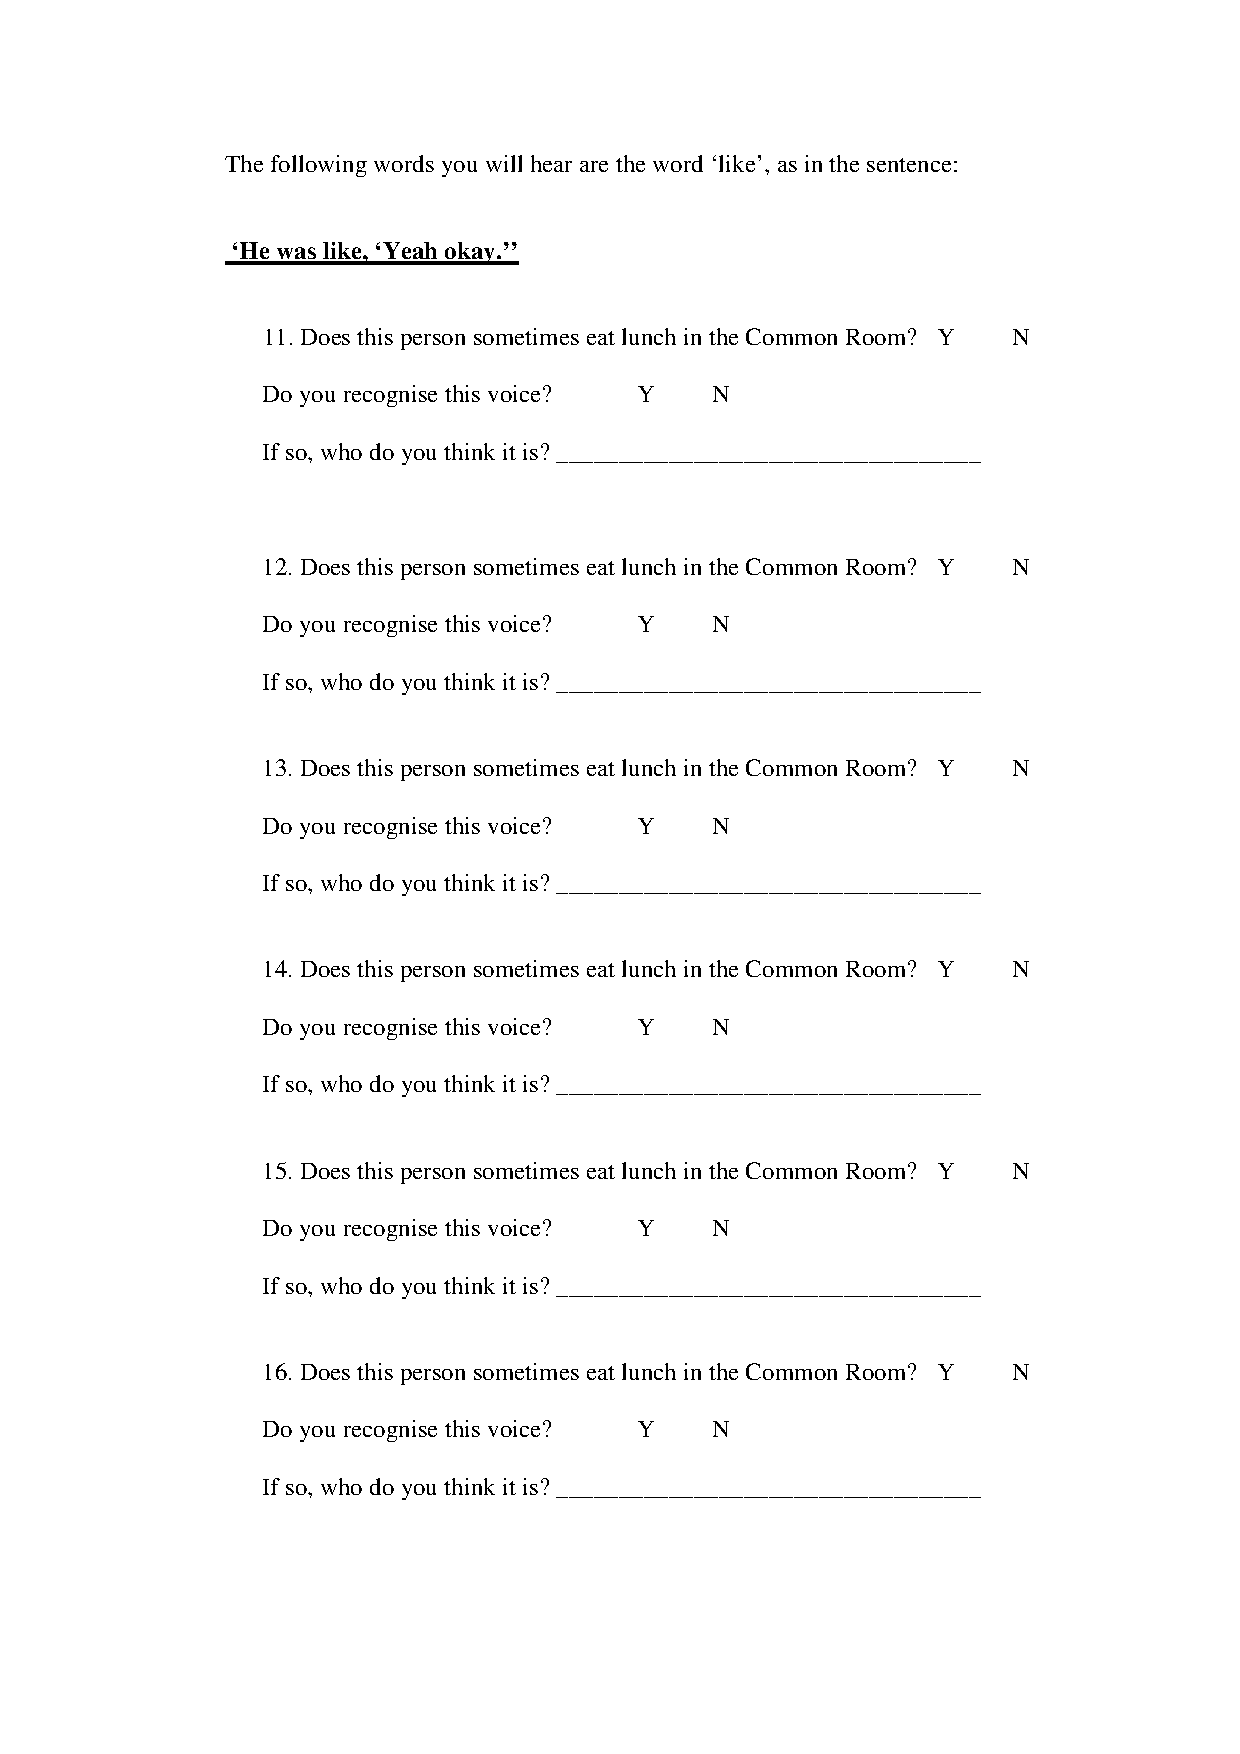
\includegraphics[width=5in]{images/Exp3page3.pdf}
		\label{x3p3}
\end{figure}

\begin{figure}
	\centering
		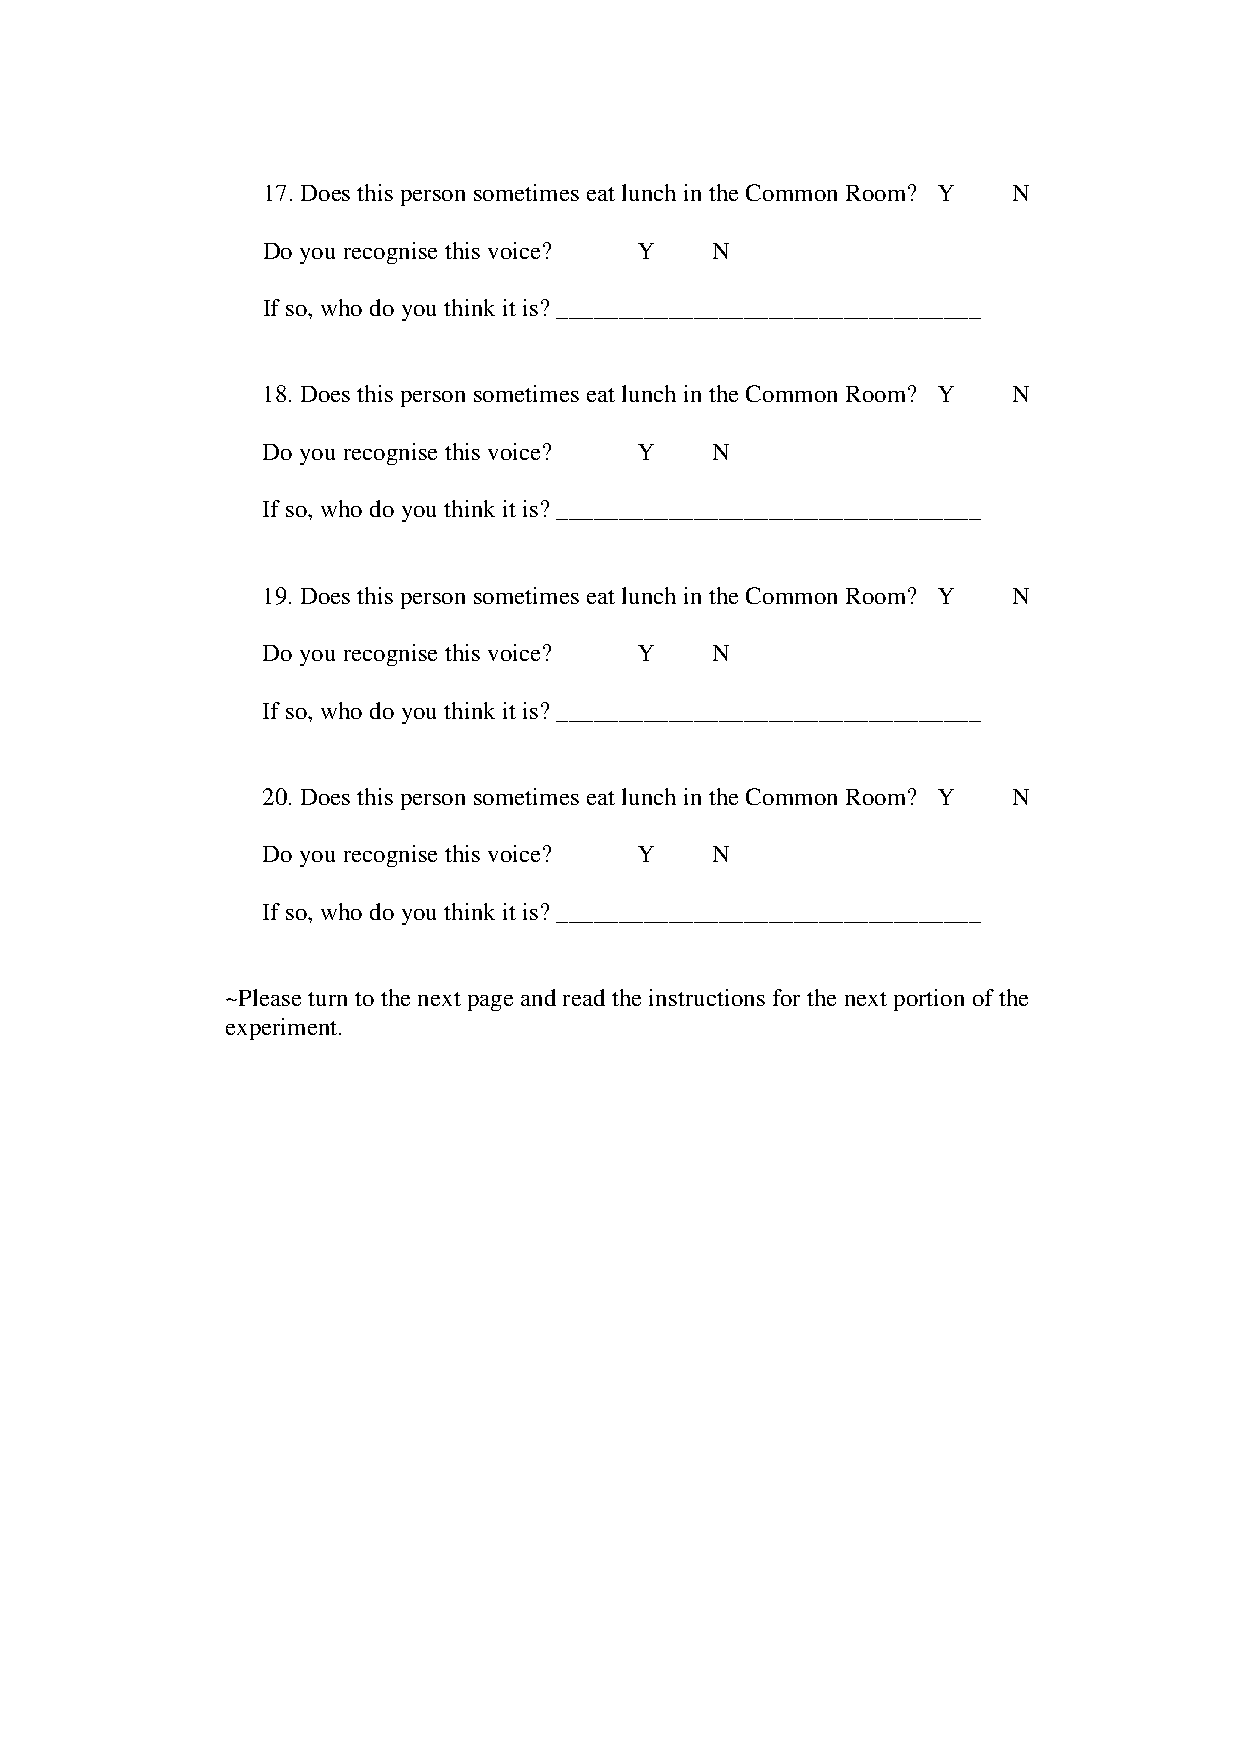
\includegraphics[width=5in]{images/Exp3page4.pdf}
		\label{x3p4}
\end{figure}

\begin{figure}
	\centering
		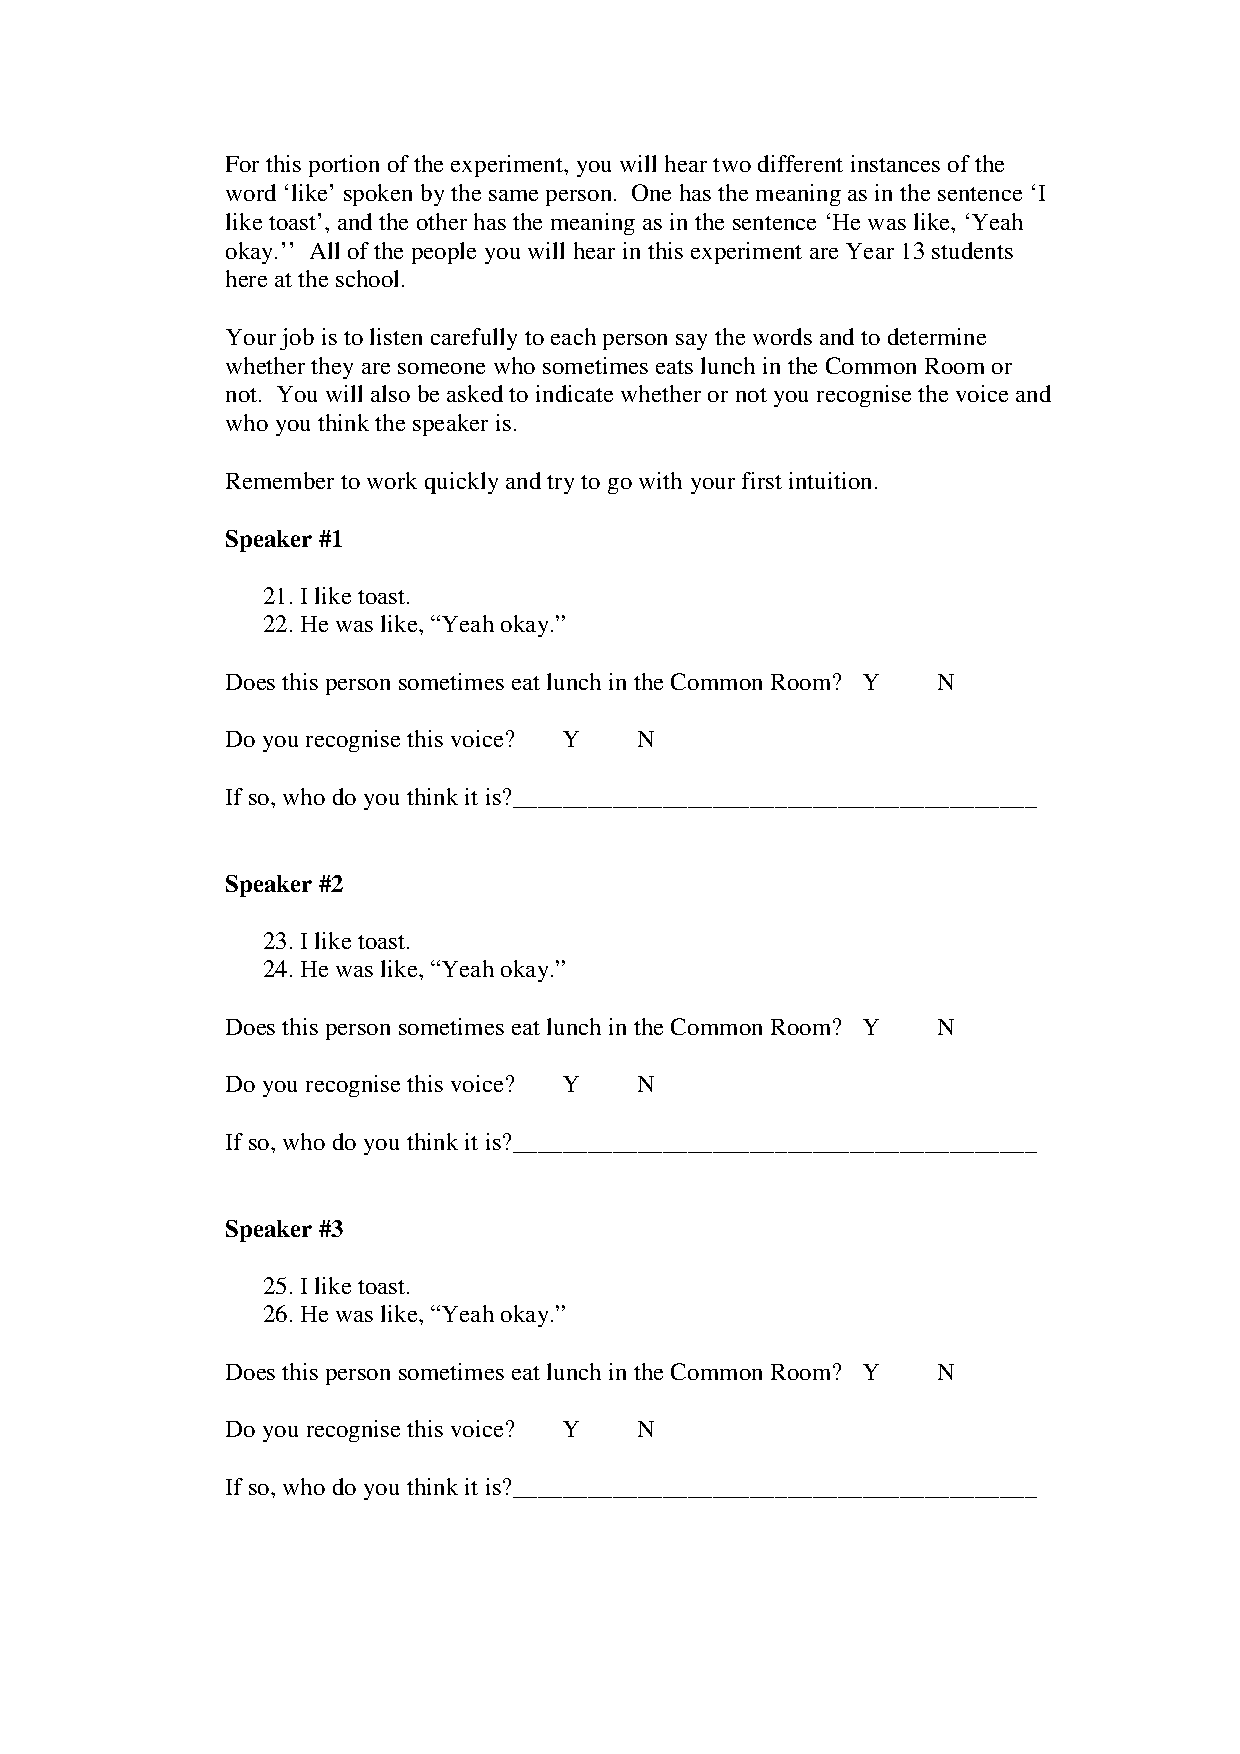
\includegraphics[width=5in]{images/Exp3page5.pdf}
		\label{x3p5}
\end{figure}

\begin{figure}
	\centering
		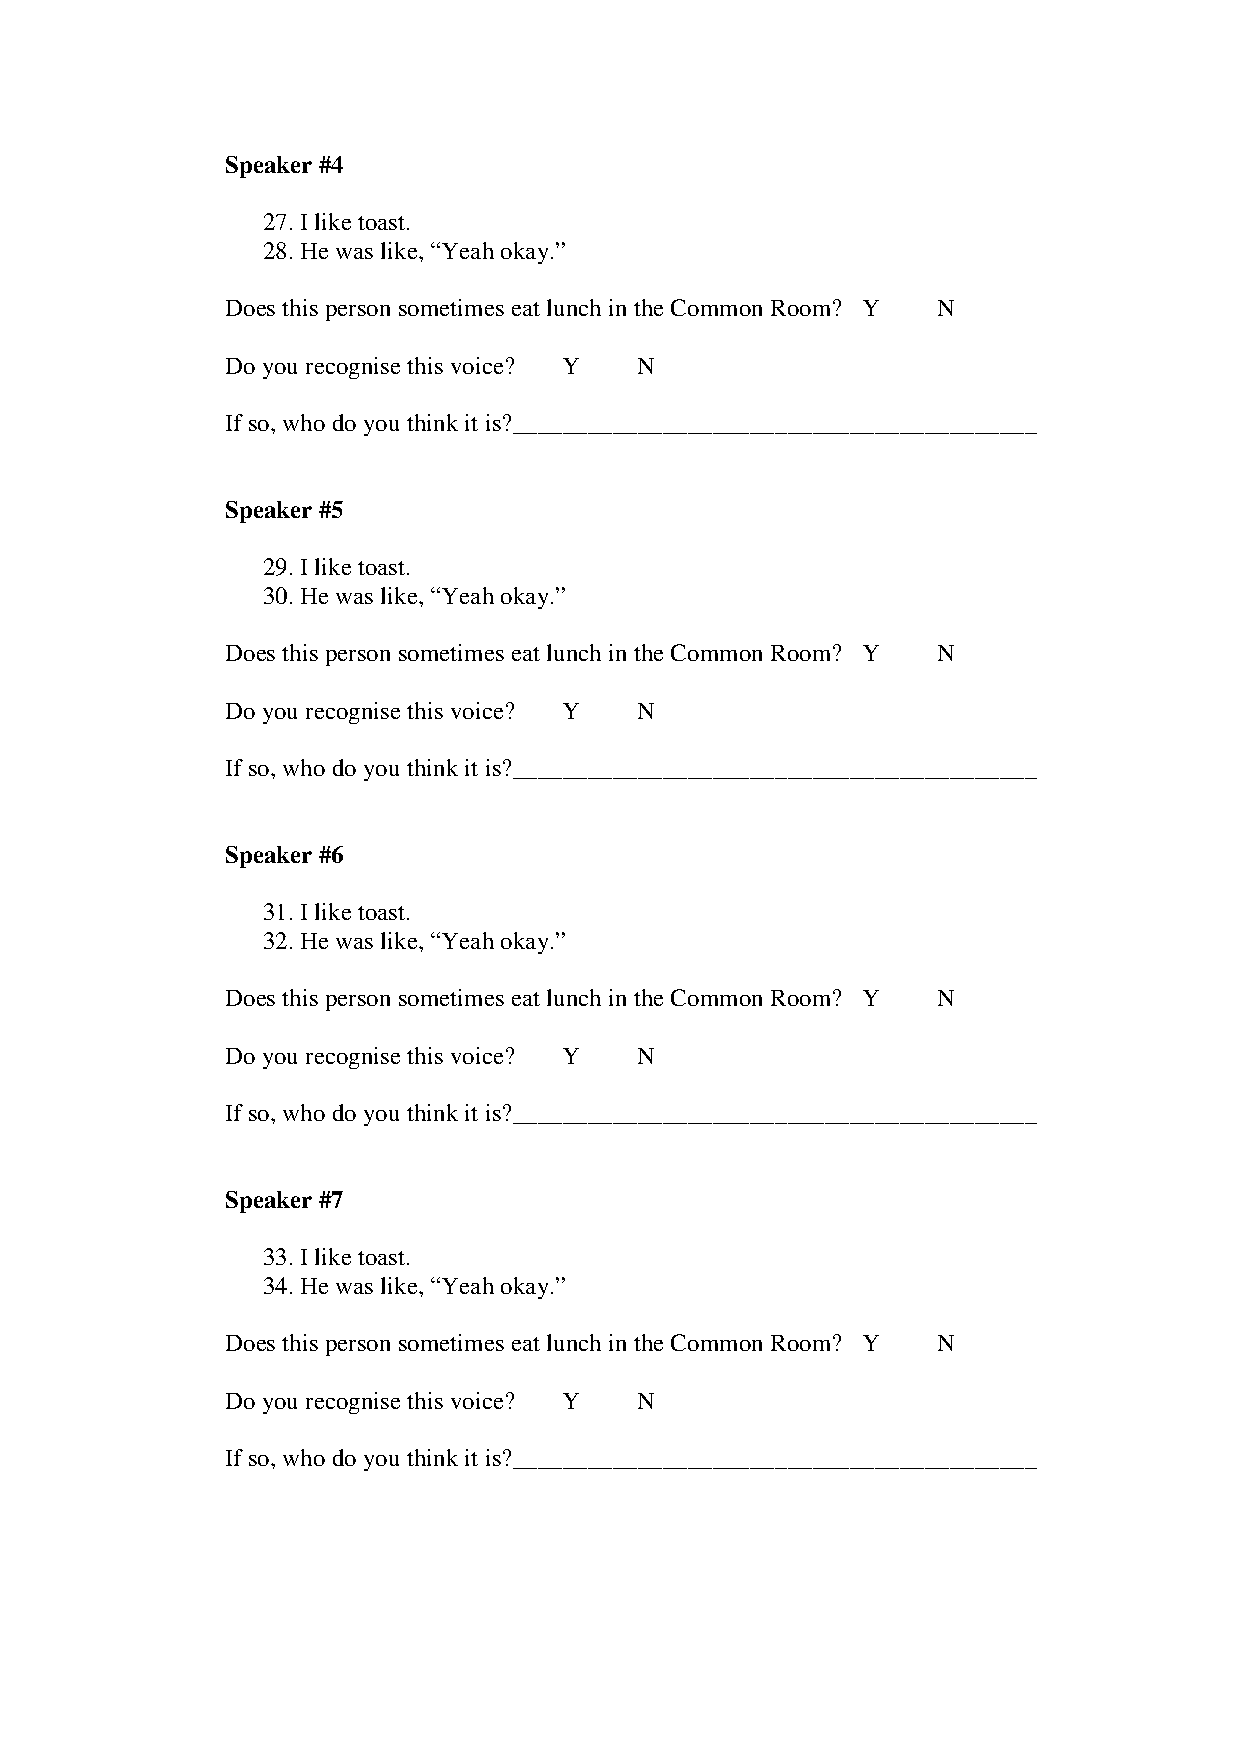
\includegraphics[width=5in]{images/Exp3page6.pdf}
		\label{x3p6}
\end{figure}

\begin{figure}
	\centering
		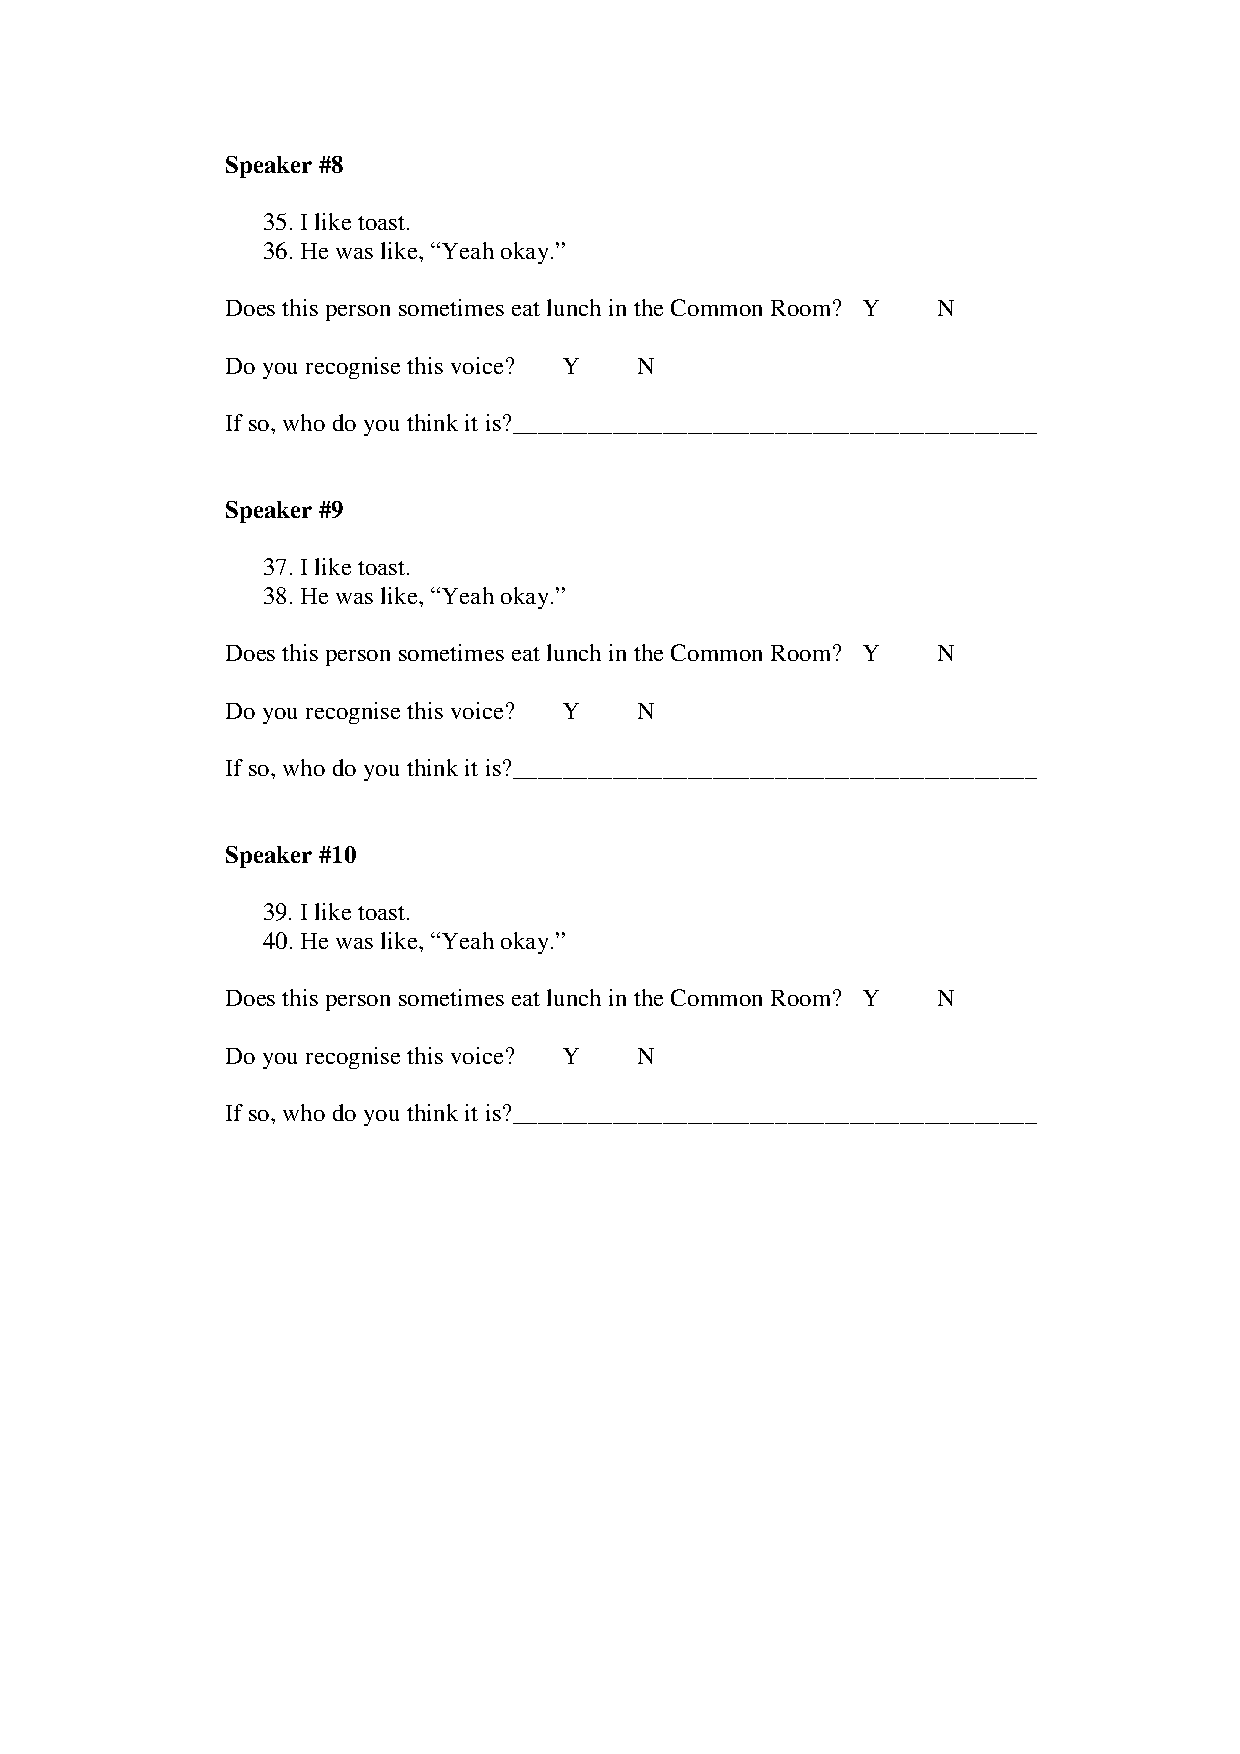
\includegraphics[width=5in]{images/Exp3page7.pdf}
		\label{x3p7}
\end{figure}



\begin{figure}[htbp]
	\centering
		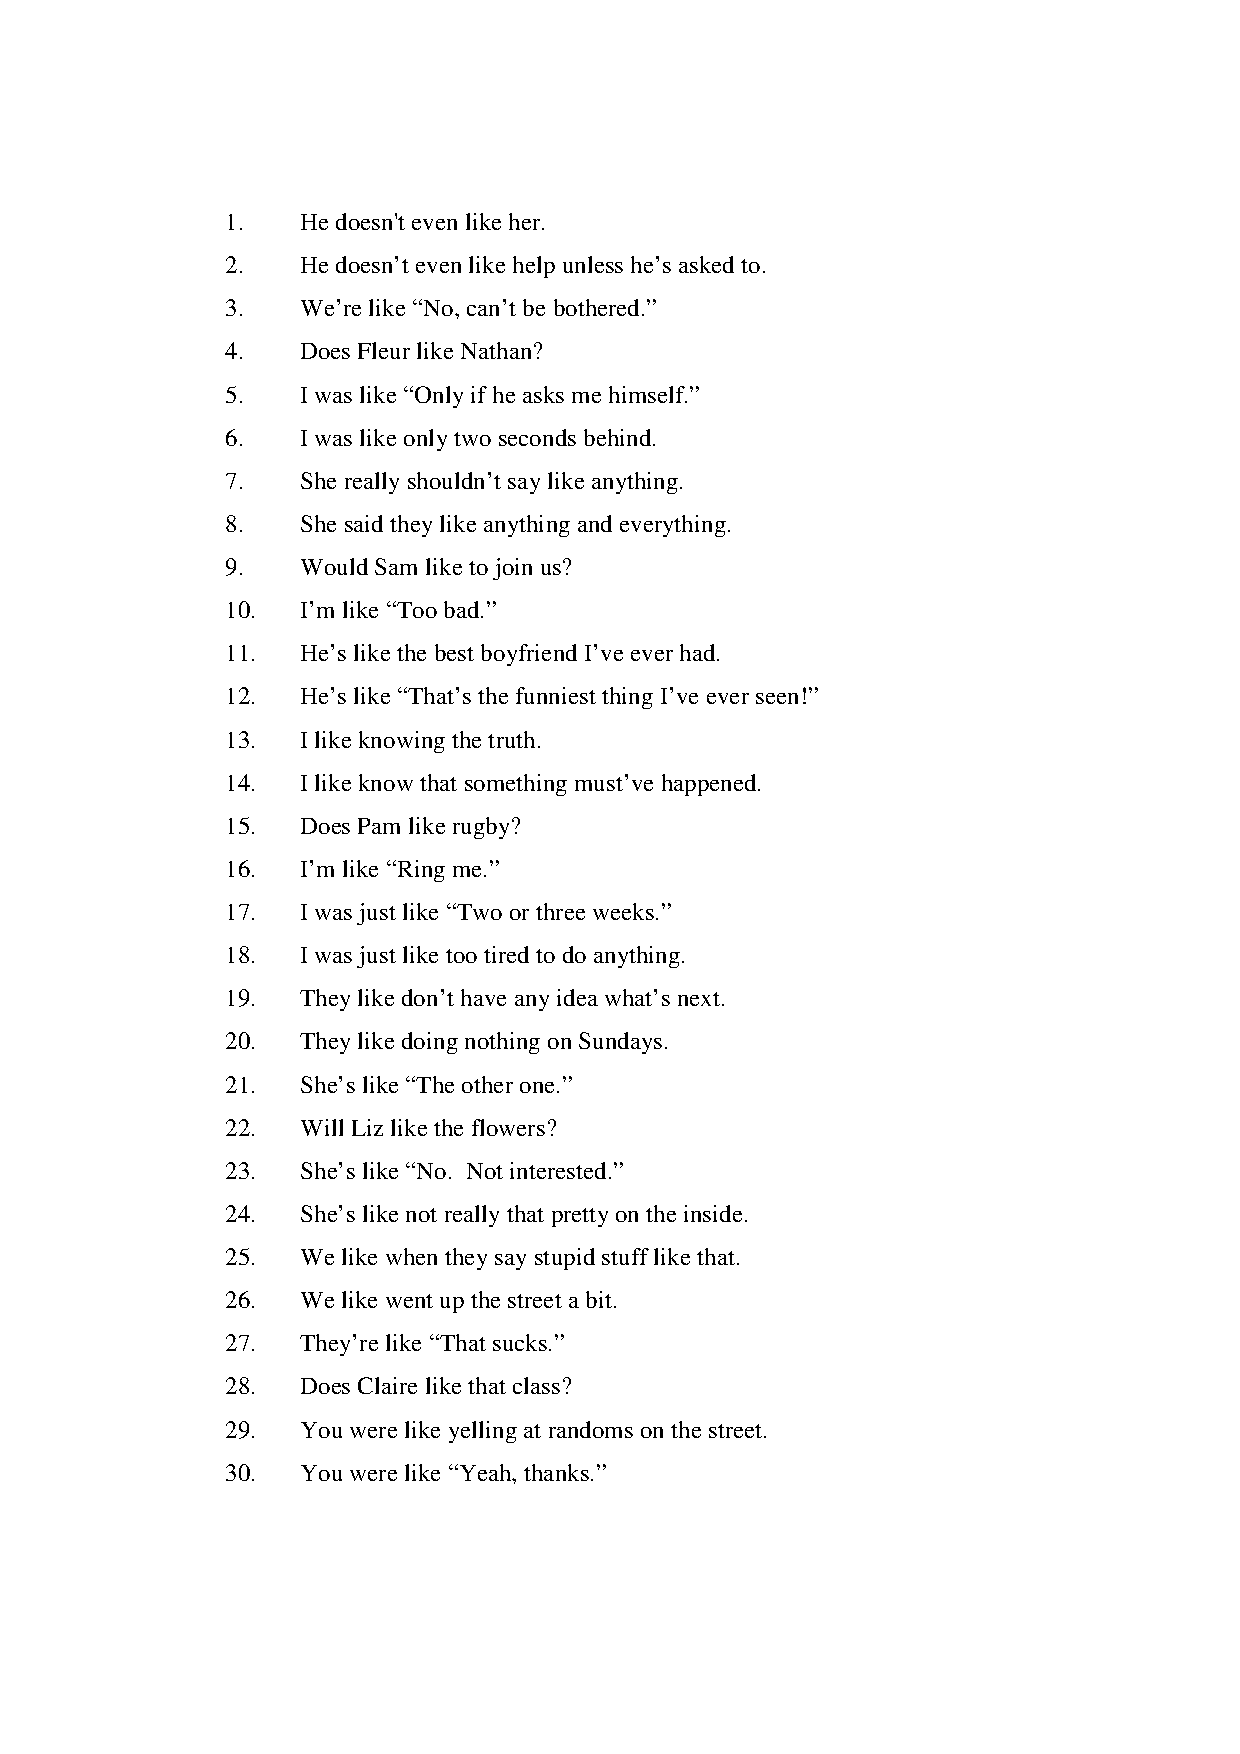
\includegraphics[width=5in]{images/ExpProductionTask.pdf}
	\caption{Production Task}
	\label{fig:ExpProductionTask}
\end{figure}




\begin{sidewaystable}[htbp]
\begin{center}
\resizebox{5in}{!}{
\begin{tabular}{llllllllll}
  \hline
  
 num.	& (N)CR &	voice	& type1 &	type2&	person &	tense	& preced.	& token1 &	token2 \\
 \hline
1	& CR	& Rose	   & d &	q	& match	& match	& match	& rose-Iwaslike1discp &	rose-Iwaslike1quote \\
2	&NCR	& Isabelle &	d &	q	& match	& match	& match	& isabelle-hewaslike1discp &	isabelle-hewaslike2quote \\
3	& CR	& Rose	   &g	&d 	   &match	& mismatch	& no info	& rose-it'slike1prep	& rose-itwaslike1discp \\
4	& CR	& Tracy	& d &	q	& mismatch & match	& likely	& tracy-he'slike1discp &	tracy-you'relike1quote \\
5	& NCR	& Isabelle &	q	& d 	& match	& mismatch & unlikely	& isabelle-shewasjustlike1quote & isabelle-she'slike1discp \\
6	& NCR	& Onya	& g	& d &	mismatch &	match	& no info	& onya-youlike1main	& onya-Ilike2discp \\
7	& CR	& Rose	& d &	q	& match	& mismatch & unlikely	& rose-itwaslike1discp	& rose-it'slike3quote \\
8	& CR	& Rachael	& d &	g &	match	& match	& match	& rachael-it'slike1discp & rachael-it'slike2prep \\
9	& NCR	& Onya & d & q & match & match & match & onya-she'slike1 & onya-she'slike1quote \\
10 & NCR & Isabelle &	d &	q	& match	& match	& match	& isabelle-shewaslike1discp	& isabelle-shewaslike1quote \\
11&	CR & Rose & g & d & mismatch	& match	& no info &	rose-Ilike1main & rose-theylike1discp \\
12 & CR & Tracy & d & q & match	& mismatch & unlikely & tracy-andtheywerelike2discp & tracy-andthey'relike1quote \\
13 & NCR & Onya & q & d & match & match & match & onya-they'relike1quote & onya2may-they'relike1 \\
14 & NCR & Isabelle & g & d & match	& match & match & isabelle-helike1main & isabelle-helike1discp \\
15 & CR & Tracy & g & d & mismatch & match & no info & tracy-Ilike1main & tracy-youlike1discp \\
16 & CR & Daphne & q & d & mismatch & match & likely & daphne-Iwaslike1quote & daphne-theywerelike1discp \\
17 & NCR & Isabelle & q & d & match & match & match & isabelle-hewaslike1quote & isabelle-hewaslike1discp \\
18 & NCR & Sarah & d & q & match & mismatch & likely & sarah-it'slike4discp	& sarah-itwaslike1quote \\
19 & CR	& Rose	& d & g & match &	match &	match &	rose-Iwaslike1discp & rose-Iwaslike1prep \\
20 & CR & Rachael & q & d & match &	match &	match &	rachael-it'sjustkindoflike1	& rachael-it'slike1discp \\
21 & NCR & Isabelle & q & d & match	& match	& match	& isabelle-shewaslike2quote	& isabelle-shewaslike1discp \\
22 & NCR & Onya & d & g &	mismatch & match & no info & onya-Ilike1discp	& onya-youlike1main  \\
23 & CR	& Rose	& d & q &	match &	mismatch & unlikely &	rose-itwaslike1discp &	rose-it'slike2quote \\
24 & NCR & Onya &	d &	q &	match &	match &	match	& onya2may-they'relike2	& onya-thegirlsarelike1quote \\
25 & CR	& Rose &	q &	d & match &	match &	match &	rose-Iwaslike2quote &	rose-Iwaslike1discp \\
26 & NCR & Onya &	q	& d &	match	& match	& match	& onya-wewerelike2 & onya-wewerelike3 \\
27 & NCR & Isabelle &	d &	g &	match	& match &	match &	isabelle-youlike1discp & isabelle-yalike1main \\
28 & CR &	Rose &	q &	d & match &	mismatch & likely &	rose-they'relike1quote	& rose-theywerelike \\
29 & CR & Tracy &	q	& d & match &	match &	match &	tracy-yourmum'slike1quote &	tracy-she'slike1discp \\
30 & CR &	Rose &	d &	q	& match	& match	& match	& rose-Iwaslike1discp & rose-Iwaslike1quote \\
31 & NCR & Onya	& d &	g	& mismatch & mismatch	& no info &	onya-Ilike3discp & onya-youlike1main \\
   \hline
   
\end{tabular}
}
\caption{The auditory stimuli played for each question in Experiment 1, listed by order played.}\label{tab:appenExp1stimuli}
\end{center}
\end{sidewaystable}	



\begin{table}[htbp]
\begin{center}
\resizebox{4.5in}{!}{
\begin{tabular}{lllllllll}
  \hline
  
num. &	(N)CR &	voice	& type1	& type2	& token1 & token2	& context1	& context2 \\
 \hline
	
1	& CR	& Rose	& g	& d	& rose-like3	& rose-discp1 & g &	d \\
2	& CR	& Rose	& q	& g	& rose-quote2	& rose-like4	& q	& g \\
3	& CR	& Rose	& d	& q	& rose-discp1	& rose-quote1	& q	& d \\
4	& CR	& Rose	& d	& g	& rose-discp5	& rose-like9	& d	& g \\
5	& CR	& Rose	& q	& g	& rose-quote4	& rose-like9	& g	& q \\
6	& CR	& Rose	& q	& d	& rose-quote2	& rose-discp2	& d	& q \\
7	& CR	& Rose	& g	& d	& rose-like10	& rose-discp6	& g	& d \\
8	& CR	& Rose	& g	& q	& rose-like3	& rose-quote1	& g	& q \\
9	& CR	& Rose	& q	& d	& rose-quote4	& rose-discp5	& q	& d \\
10	& CR	& Rose	& g	& d	& rose-like8	& rose-discp3 &	d	& g \\
11	& CR	& Rose	& g	& q	& rose-like8	& rose-quote3	& q	& g \\
12	& CR	& Rose	& d	& q	& rose-discp6	& rose-quote5	& q	& d \\
13	& CR	& Rose	& d	& g	& rose-discp2	& rose-like4	& g	& d \\
14	& CR	& Rose	& g	& q	& rose-like10	& rose-quote5	& q	& g \\
15	& CR	& Rose	& d	& q	& rose-discp3	& rose-quote3	& d	& q \\
16	& NCR	& Meredith	& g	& d	& meredith-like1main	& meredith-like1discp	& d	& g \\
17	& NCR	& Meredith	& g	& q	& meredith-like5main	& meredith-like5quote	& g	& q \\
18	& NCR	& Meredith	& q	& d	& meredith-like2quote	& meredith-like2discp	& d	& q \\
19	& NCR	& Meredith	& d	& g	& meredith-like4discp	& meredith-like4main	& d	& g \\
20	& NCR	& Meredith	& g	& q	& meredith-like1main	& meredith-like1quote	& g	& q \\
21	& NCR	& Meredith	& d	& q	& meredith-like1discp	& meredith-like1quote	& d	& q \\
22	& NCR	& Meredith	& g	& d	& meredith-like5main	& meredith-like5discp	& g	& d \\
23	& NCR	& Meredith	& q	& g	& meredith-like2quote	& meredith-like2main	& g	& q \\
24	& NCR	& Meredith	& q	& d	& meredith-like4quote	& meredith-like4discp	& q	& d \\
25	& NCR	& Meredith	& g	& d	& meredith-like3main	& meredith-like3discp	& d	& g \\
26	& NCR	& Meredith	& g	& q	& meredith-like3main	& meredith-like3quote	& q	& g \\
27	& NCR	& Meredith	& d	& q	& meredith-like3discp	& meredith-like3quote	& d	& q \\
28	& NCR	& Meredith	& d	& g	& meredith-like2discp	& meredith-like2main	& g	& d \\
29	& NCR	& Meredith	& q	& g	& meredith-like4quote	& meredith-like4main	& q	& g \\
30	& NCR	& Meredith	& d	& q	& meredith-like5discp	& meredith-like5quote	& q	& d \\
31	& CR	& Tracy	& d	& g	& tracy-discp1	& tracy-like1	& g	& d \\
32	& CR	& Tracy	& q	& g	& tracy-quote1	& tracy-like1	& g	& q \\
33	& CR	& Tracy	& d	& q	& tracy-discp2	& tracy-quote2	& d	& q \\
34	& CR	& Tracy	& g	& d	& tracy-like4	& tracy-discp4	& d	& g \\
35	& CR	& Tracy	& q	& g	& tracy-quote3	& tracy-like3	& q	& g \\
36	& CR	& Tracy	& q	& d	& tracy-quote1	& tracy-discp1 &	q &	d \\
37	& CR	& Tracy	& d	& g	& tracy-discp3	& tracy-like3	& d	& g \\
38	& CR	& Tracy	& g	& q	& tracy-like4	& tracy-quote4	& g	& q \\
39	& CR	& Tracy	& q	& d	& tracy-quote5	& tracy-discp5	& q	& d \\
40	& CR	& Tracy	& d	& g	& tracy-discp5	& tracy-like5	& g	& d \\
41	& CR	& Tracy	& g	& q	& tracy-like2	& tracy-quote2	& q	& g \\
42	& CR	& Tracy	& q	& d	& tracy-quote3	& tracy-discp3	& d	& q \\
43	& CR	& Tracy	& g	& d	& tracy-like2	& tracy-discp2	& g	& d \\
44	& CR	& Tracy	& q	& g	& tracy-quote5	& tracy-like5	& q	& g \\
45	& CR	& Tracy	& d	& q	& tracy-discp4	& tracy-quote4	& q	& d \\
46	& NCR	& Onya	& d	& g	& onya-discp1	& onya- like6	& g	& d \\
47	& NCR	& Onya	& q	& g	& onya-quote1	& onya- like6	& g	& q \\
48	& NCR	& Onya	& d	& q	& onya-discp2	& onya-quote2	& d	& q \\
49	& NCR	& Onya	& g	& d	& onya- like9	& onya-discp4	& d	& g \\
50	& NCR	& Onya	& g	& q	& onya- like7	& onya-quote2	& g	& q \\
51	& NCR	& Onya	& q	& d	& onya-quote1	& onya-discp1	& q	& d \\
52	& NCR	& Onya	& d	& g	& onya-discp5	& onya- like10	& d	& g \\
53	& NCR	& Onya	& g	& q	& onya- like9	& onya-quote4	& q	& g \\
54	& NCR	& Onya	& d	& q	& onya-discp4	& onya-quote4	& q	& d \\
55	& NCR	& Onya	& d	& g	& onya-discp3	& onya- like8	& d	& g \\
56	& NCR	& Onya	& q	& g	& onya-quote3	& onya- like8	& q	& g \\
57	& NCR	& Onya	& q	& d	& onya-quote5 &	onya-discp5	& d	& q \\
58	& NCR	& Onya	& g	& d	& onya- like7	& onya-discp2	& g	& d \\
59	& NCR	& Onya	& q	& g	& onya-quote5	& onya- like10	& g	& q \\
60	& NCR	& Onya	& q	& d	& onya-quote3	& onya-discp3	& d	& q \\

   \hline
   
	\end{tabular}
}
	\caption{The auditory stimuli played for each question in Experiment 2, listed by order played.}\label{tab:appenExp2stimuli}
	\end{center}
\end{table}	





\begin{table}[htbp]
\begin{center}
\resizebox{4.5in}{!}{
\begin{tabular}{llllllll}
  \hline
  
task & num. & (N)CR &	voice	& type1	& type2	& token1 & token2	\\
 \hline
 
 1 & 1 & CR & Anita & g & na & anita-like1 & na \\
 1 & 2 & NCR & Vanessa & g & na & vanessa-like1 & na \\
 1 & 3 & NCR & Onya & g & na & onya-like6 & na \\
 1 & 4 & CR & Rose & g & na & rose-like9 & na \\
 1 & 5 & NCR & Meredith & g & na & meredith-like1 & na \\
 1 & 6 & CR & Rachel & g & na & rachel-like1 & na \\
 1 & 7 & CR & Tracy & g & na & tracy-like2 & na \\
 1 & 8 & NCR & Isabelle & g & na & isabelle-like2 & na \\
 1 & 9 & CR & Betty & g & na & betty-like1 & na \\
 1 & 10 & NCR & Sarah & g & na & sarah-like1 & na \\
 2 & 11 & NCR & Isabelle & q & na & isabelle-quote5 & na \\
 2 & 12 & NCR & Onya & q & na & onya-quote4 & na \\
 2 & 13 & CR & Rose & q & na & rose-quote2 & na \\
 2 & 14 & NCR & Sarah & q & na & sarah-quote1 & na \\
 2 & 15 & CR & Rachel & q & na & rachael-quote1 & na \\
 2 & 16 & CR & Betty & q & na & betty-quote1 & na \\
 2 & 17 & NCR & Vanessa & q & na & vanessa-quote1 & na \\
 2 & 18 & CR & Anita & q & na & anita-quote2 & na \\
 2 & 19 & NCR & Meredith & q & na & meredith-quote6 & na \\
 2 & 20 & CR & Tracy & q & na & tracy-quote1 & na \\
 3 & 21-22 & CR & Betty & g & q & betty-like1 & betty-quote1 \\
 3 & 23-24 & NCR & Isabelle & g & q & isabelle-like2 & isabelle-quote5 \\
 3 & 25-26 & CR & Rose & g & q & rose-like9 & rose-quote2 \\
 3 & 27-28 & NCR & Onya & g & q & onya-like6 & onya-quote4 \\
 3 & 29-30 & CR & Rachel & g & q & rachel-like1 & rachel-quote1 \\
 3 & 31-32 & NCR & Sarah & g & q & sarah-like1 & sarah-quote1 \\
 3 & 33-34 & CR & Tracy & g & q & tracy-like2 & tracy-quote1 \\
 3 & 35-36 & NCR & Vanessa & g & q & vanessa-like1 & vanessa-quote1 \\
 3 & 37-38 & CR & Anita & g & q & anita-like1 & anita-quote2 \\
 3 & 39-40 & NCR & Meredith & g & q & meredith-like1 & meredith-quote6 \\
 
    \hline
   
	\end{tabular}
}
	\caption{The auditory stimuli played for each question in Experiment 3, listed by order played.}\label{tab:appenExp3stimuli}
	\end{center}
\end{table}	